\documentclass{article}
\usepackage{fullpage}
%\usepackage{nips_2018}

%\usepackage{comment}
%\usepackage{natbib}

\usepackage{extarrows}
%% BEAUTIFY
\setlength\parindent{0pt}
\setlength{\parskip}{1em}
\usepackage[sc]{mathpazo} % Use the Palatino font
\usepackage[T1]{fontenc}  % Use 8-bit encoding that has 256 glyphs
\linespread{1.05}         % Line spacing - Palatino needs more space between lines
\usepackage{microtype}    % Slightly tweak font spacing for aesthetics
\usepackage{abstract}     % Allows abstract customization
\renewcommand{\abstractnamefont}{\normalfont\bfseries}      % Set the "Abstract" text to bold
\renewcommand{\abstracttextfont}{\normalfont\small\itshape} % Set the abstract itself to small italic text
 \usepackage{titlesec}     % Allows customization of titles
% \renewcommand\thesection{\Roman{section}} % Roman numerals for the sections
% \renewcommand\thesubsection{\Roman{subsection}} % Roman numerals for subsections
 \titleformat{\section}[block]{\large\scshape\centering}{\thesection.}{1em}{} % Change the look of the section titles
 \titleformat{\subsection}[block]{\large}{\thesubsection.}{1em}{} % Change the look of the section titles


%%%%%%%%%%%%%%%%%%%
% CUSTOM PACTAGES %
%%%%%%%%%%%%%%%%%%%
\usepackage{wrapfig}
\usepackage{amsmath,amssymb,mathtools}
\usepackage{bm}
\usepackage{amsthm}
\usepackage{graphicx,subfig,color,wrapfig,epsfig,epstopdf}
\usepackage{enumitem}
\usepackage{booktabs}
% For algorithms
\usepackage{algorithm,algorithmic}

\renewcommand{\paragraph}[1]{\noindent\textbf{#1}}

%%%%%%%%%%%%%%%%%%%

% to compile a camera-ready version, add the [final] option, e.g.:
% \usepackage[final]{nips_2017}

%\usepackage[utf8]{inputenc} % allow utf-8 input
%\usepackage[T1]{fontenc}    % use 8-bit T1 fonts
%\usepackage{hyperref}       % hyperlinks
%\usepackage{cleveref}
%\usepackage{url}            % simple URL typesetting
%\usepackage{booktabs}       % professional-quality tables
%\usepackage{amsfonts}       % blackboard math symbols
%\usepackage{nicefrac}       % compact symbols for 1/2, etc.
%\usepackage{microtype}      % microtypography

\usepackage[utf8]{inputenc} % allow utf-8 input
\usepackage[T1]{fontenc}    % use 8-bit T1 fonts
\usepackage{hyperref}       % hyperlinks
\usepackage{url}            % simple URL typesetting
\usepackage{booktabs}       % professional-quality tables
\usepackage{amsfonts}       % blackboard math symbols
\usepackage{nicefrac}       % compact symbols for 1/2, etc.
\usepackage{microtype}      % microtypography

\usepackage{color}
\def\rc{\color{red}}

% I am too lazy to add nonumber
\newcommand\numberthis{\addtocounter{equation}{1}\tag{\theequation}}

\allowdisplaybreaks[4]

% Theorem
\newcounter{ass_counter}
\newcounter{thm_counter}
\newcounter{remark_counter}
% \newtheorem{proposition}[thm_counter]{Proposition}%[section]
\newtheorem{theorem}[thm_counter]{Theorem}%[section]
\newtheorem{lemma}[thm_counter]{Lemma}%[Lemma]
\newtheorem{corollary}[thm_counter]{Corollary}
\newtheorem{assumption}[ass_counter]{Assumption}
\newtheorem{remark}[remark_counter]{Remark}
%\Crefname{assumption}{Assumption}{Assumptions}

%\usepackage[utf8]{inputenc} % allow utf-8 input
%\usepackage[T1]{fontenc}    % use 8-bit T1 fonts
%\usepackage{hyperref}       % hyperlinks
%\usepackage{url}            % simple URL typesetting
%\usepackage{booktabs}       % professional-quality tables
%\usepackage{amsfonts}       % blackboard math symbols
%\usepackage{nicefrac}       % compact symbols for 1/2, etc.
%\usepackage{microtype}      % microtypography
%\usepackage{color}

\usepackage{amsmath,amssymb,mathtools}
\usepackage{bm}
\usepackage{amsthm}
\usepackage{graphicx,subfig,color,wrapfig,epsfig,epstopdf}
\usepackage{enumitem}
\usepackage{booktabs}
% For algorithms
\usepackage{algorithm,algorithmic}

\newcommand{\todo}[1]{\textcolor{red}{\textbf{TODO:{#1}}}}

\DeclareMathOperator{\Tr}{Tr}

\title{Decentralized Learning over {\rc Unstable Networks}}

% The \author macro works with any number of authors. There are two
% commands used to separate the names and addresses of multiple
% authors: \And and \AND.
%
% Using \And between authors leaves it to LaTeX to determine where to
% break the lines. Using \AND forces a line break at that point. So,
% if LaTeX puts 3 of 4 authors names on the first line, and the last
% on the second line, try using \AND instead of \And before the third
% author name.

\author{
  Dummy Author \\
  \texttt{email@address} \\
  %% examples of more authors
  %% \And
  %% Coauthor \\
  %% Affiliation \\
  %% Address \\
  %% \texttt{email} \\
  %% \AND
  %% Coauthor \\
  %% Affiliation \\
  %% Address \\
  %% \texttt{email} \\
  %% \And
  %% Coauthor \\
  %% Affiliation \\
  %% Address \\
  %% \texttt{email} \\
  %% \And
  %% Coauthor \\
  %% Affiliation \\
  %% Address \\
  %% \texttt{email} \\
}

\begin{document}
% \nipsfinalcopy is no longer used

\maketitle

\begin{abstract}
Most of today's distributed machine learning systems
are built upon {\em reliable networks}: whenever
two machines exchange information (e.g., gradients
or models), the network layer guarantees the delivery
of a given message. On the other hand, recent machine
work exhibits several examples of
the impressive error tolerance of machine learning algorithms. In this paper, we start from the 
following question: {\em Can we design machine
learning systems that are tolerant to network unreliability during training?}

With this motivation, we focus on a theoretical
problem that is of independent interest: assuming
$N$ machines, each of which holds a partition
of the data and runs a local 
stochastic gradient algorithm, if every iteration
a (different) random subset of machines 
average their model, can we still converge towards the  
same global model as standard distributed 
learning algorithm? In the context of
prior arts, this problem can be phrased as
{\em decentralized learning algorithm over
a random topology}. The technical contribution of this
paper is a novel theoretical analysis to prove 
that 
the decentralized learning over random topologies can achieve comparable convergence rate of both centralized learning or decentralized learning, and we also proved that the influence of the package drop rate would diminish with the growth of the workers number.
We map this theoretical result to a real-world
scenario of training deep neural networks over
unreliable networks, and conduct network simulation
to validate potential system improvement by allowing
the networks to be unreliable.
\end{abstract}

% \vspace{-0.5em}
\section{Introduction}
% \vspace{-1em}

Distributed learning has attracted significant interest from both
academia and industry. Over the last decade, researchers have 
come with up a range of different designs of more efficient 
learning systems. An important subset of this work focuses on 
understanding the impact of different system relaxations to
the convergence and performance of distributed stochastic gradient
descent, such as the compression of communication, e.g~\cite{seide2016cntk},
decentralized communication~\cite{lian2017can,sirb2016consensus,lan2017communication}, and asynchronous
communication~\cite{lian2017asynchronous,zhang2013asynchronous,lian2015asynchronous}. 
Most of these works are motivated by real-world system bottlenecks, abstracted as general problems for the purposes of analysis.

In this paper, we are motivated by another interesting potential system relaxation---the reliability of the communication channel. We formalize this theoretical problem,   and conduct a novel
convergence analysis for such a scenario. Specifically, we focus on the case where the communication channel between any two machines has a probability $p$ of not delivering the messages (which may be a full gradient update, or just part of it). 
This setting can be abstracted as the simple, general problem of learning in a decentralized multi-node system, over a random topology that changes upon every single communication.

More precisely, we assume a standard real-world system
implementation which uses Reduce-Scatter and All-Gather primitives for aggregating gradients or models, executing standard data-parallel stochastic gradient descent (SGD). 
In a nutshell, the algorithm, which we call RSAG, is as follows. Given
$N$ machines, each machine runs its local SGD step.
At every communication step, machines may exchange their {\em local models}. 
Aggregation is performed as follows: the model is partitioned into $N$ blocks, one per node; for each blocks $i$, (corresponding to the Reduce-Scatter Step) a uniformly random 
subset of machines average their
model on block $i$, and then, (in the All-Gather Step) propagate the average to a uniformly 
random subset of machines and update the block $i$ of their local model.
Machines not chosen for the Reduce-Scatter step
do not contribute to the average, and all machines that are not chosen  for the All-Gather will not receive updates on their model block $i$.
This is a realistic model of running a AllReduce operator implemented
with Reduce-Scatter/All-Gather on unreliable network.

Our main technical contribution is characterizing the convergence properties of the RSAG algorithm. To the best of our knowledge, this is a novel
theoretical analysis of such a faulty-communication model. Compared with previous work on
decentralized learning, this paper considers the impact
of a random topology on convergence. Specifically, we prove that the decentralized learning over random topologies can converge as efficient as the decentralized learning, over a fixed topology and admit linear speedup property. Moreover, we also proved that the affection of the package drop rate would diminish while the number of the workers becomes more and more.

We apply our theoretical result to a real-world use case,
illustrating the potential benefit of allowing an unreliable network. We focus on network sharing among multiple applications---a scenario where the machine learning algorithms are training using 
GPUs and another service, is using computation on the same set of machines. Both applications communicate using the same network. In this case, if the machine learning traffic is tolerant to some losses, the other application can potentially be made faster by receiving priority for its network traffic. Through network simulations, we find that tolerating a $10\%$ drop rate for the learning traffic can make a simple (emulated) Web service up to $1.2\times$ faster
(In this application even small speedups of $10\%$ are significant for such services; for example, Google actively pursues minimizing its Web services' response latency ). This degree of loss of learning traffic does not impact convergence rate for a range of machine learning applications such as training ResNet for image datasets and training LSTM for natural language datasets.

% \vspace{-0.5em}
\section{Related Work}
% \vspace{-1em}

\footnote{\rc To Chen and Hanlin: we need more comprehensive literature review. You can refer the review from NIPS.}

There has been a significant work on distributing deep learning, e.g.~\cite{seide2016cntk,abadi2016tensorflow,goyal2017accurate}. Due to space constraints, we only mainly focus on work considering data-parallel SGD with randomized communication. 

\paragraph{Gossip-like Communications} The most related to this
paper is a line of work considering gossip-like communication
patterns for distributed learning. 
Specifically,~\cite{jin2016scale} proposes to scale the gradient aggregation process via a gossip-like mechanism. Reference~\cite{blot2016gossip} considers a more radical approach, called GoSGD, where each node exchanges gradients with a random subset of other nodes in each round. They show that GoSGD can be faster than Elastic Averaging SGD~\cite{zhang2015deep} on CIFAR-10, but provide no large-scale experiments or theoretical justification. 
Recently,~\cite{daily2018gossipgrad} proposed GossipGrad, a more complex gossip-based scheme with upper bounds on the time for nodes to communicate indirectly, periodic rotation of partners and shuffling of the input data, which provides strong empirical results on large-scale deployments. 
The authors also provide an informal justification for why GossipGrad should converge. Despite the promising empirical results, there is very little known in terms of convergence guarantees. 


\paragraph{Random topology decentralized algorithms} In \cite{boyd2006randomized}, a randomized decentralized SGD is studied. The weighted matrix for randomized algorithms can be time-varying, which means workers are allowed to change the communication network based on the availability of the network. Our work is also a variant of randomized decentralized SGD, since the weighted matrix for communication is unpredictable due to package loss. However, we do not require the weighted matrix to be doubly stochastic, which cannot always be satisfied in practical, and we also proved that our algorithm is more feasible for a larger network. 


\paragraph{AllReduce SGD and Decentralized Learning} The overcome to limitation of the parameter-server model, another approach, called all-reduced SGD is proposed\cite{iandola2016firecaffe}. It admits a all-to-all topology for information communication, each worker in the network would communicate to all others\cite{tang2018d}. This papers builds upon an 
AllReduce communication pattern but focus on the scenario that
there are message losses in the network layer.

Another direction of related work considers decentralized learning over \emph{fixed}, but incomplete graph topologies. A recent result by~\cite{lian2017can} provided strong convergence bounds for a similar algorithm to the one we are considering, in a setting where the communication graph is fixed and regular. Here, we consider random, dynamically changing topologies, and therefore require a different analytic approach. 



%\section{Algorithms}
%
%We denote $n$ to be the number of working nodes.
%
%We proof and conduct experiments on a data distributed variant of the \textit{stochastic gradient descent} algorithm. Every node $i$ has a partition of the data initially and maintains a local copy of the current model $x_i^t$ at time $t$. Concurrently, each node $i$ samples a random element $\bm{\xi}_i^t$  based on which it calculates a stochastic gradient $\nabla F_i\left(x_i^t, \bm{\xi}_i^t \right)$.
%
%We distinguish between two different aggregation strategies:
%
%\begin{enumerate}
%    \item \textbf{Gradient Averaging:} The average of all the stochastic gradients is calculated and used to update the model:
%    \[
%    x_i^{t+1} = x_i^t - \gamma \frac{1}{n}\sum_{i = 1}^{n}\nabla F_i\left(x_i^t, \bm{\xi}_i^t \right).
%    \]
%    \item \textbf{Model Averaging:} The model variables are averaged after having performed the update locally:
%    \[
%    x_i^{t+1} = \frac{1}{n}\sum_{i = 1}^{n}\left(x_i^t - \gamma \nabla F_i\left(x_i^t, \bm{\xi}_i^t \right)\right)
%    \]
%\end{enumerate}
%
%$\gamma$ represents the learning rate in both variants. Both methods ensure that all the nodes will have the same model at time $t+1$. The fundamental difference between those two algorithms lies in the point in time, at which data is exchanged and averaged across all the nodes. In both cases, the sum operator for averaging can be implemented as an \textit{AllReduce} operation.
%
%
%\begin{algorithm}[t]
%\scriptsize
%
%\caption{ICP-DSGD - Gradient Averaging}\label{alg2}
%\begin{minipage}{1.0\linewidth}
%\small
%\begin{algorithmic}[1]
%\STATE {\bfseries Input:} Initial point $\bm{x}^{(i)}_1=\bm{x}_1$, iteration step length $\gamma$, confusion matrix $W$, and number of total iterations T.
%\FOR{$t = 1,2,\cdots,T$}
%\STATE Randomly sample $\bm{\xi}^{(i)}_t$ from local data of the $i$th node
%\STATE Compute a local stochastic gradient based on $\bm{\xi}^{(i)}_t$ and current optimization variable $\bm{x}^{(i)}_t:\nabla F^{(i)}(\bm{x}^{(i)}_t,\bm{\xi}^{(i)}_t)$
%\STATE Set vector locally
%\[
%\bm{v}_{t}^{(i)}\gets \nabla F^{(i)}(\bm{x}^{(i)}_t,\bm{\xi}^{(i)}_t)
%\]
%and divide $\bm{v}^{(i)}_t$ into $n$ partial vector $\tilde{\bm{v}}_t^{(i\to j)}$ where $j \in \{1,\dots,n\}$.
%\STATE Each worker $i$ assign the partial vector $\tilde{\bm{v}}_t^{(i\to j)}$ to all the other workers, denote as worker $j$, in the network. Then each worker finish the summation using the partial vector using
%\begin{align*}
%\tilde{\bm{v}}^{(i)}_t = \frac{1}{n}\sum_{j=1}^n\tilde{\bm{v}}_t^{(j\to i)}.
%\end{align*}
%\STATE Each worker broadcast $\tilde{\bm{v}}^{(i)}_t$ to all others and sets each value of $\bm{v}_{t}^{(i)}$ based on the partial vector received in $\tilde{\bm{v}}^{(j)}_t$ for $j \in \{1,\dots,n\}$.
%
%\begin{align*}
%\bm{x}_{t+1}^{(i)} = \bm{x}_t^{(i)} - \gamma\bm{v}_{t}^{(i)}
%\end{align*}
%
%\ENDFOR
%\STATE {\bfseries Output:} $\bm{x}^{(i)}_T$
%\end{algorithmic}
%\end{minipage}
%\end{algorithm}
%
%\subsection{AllReduce}
%
%AllReduce algorithms are run with any binary operation (in our case \textit{sum}) over multiple vectors. Assume that every node $i$ has a local vector $v_i \in \mathbb{R}^d$. On naive way of implementing an AllReduce is to collect all the vectors on a distinct node, let this one calculate the sum of all the vector $\sum_{i = 1}^{n}v_i$, and broadcast the result back to all the other nodes. This is known to be a Parameter-Server paradigm.
%
%In order to prevent this server node to become the network bottleneck, we split the algorithm into two parts: \textit{Reduce-Scatter} and \textit{AllGather}. For the Reduce-Scatter, the dimension of the vector space $d$ is uniformly partitioned into $n$ parts, each having size $\frac{d}{n}$. Every node is responsible the reduce a distinct part of the entire result. Therefore, the part of the vector is directly sent from every node to its intended recipient. After having performed a local reduction in parallel, all the nodes need to exchange and gather the rest of the vector. This task is called an AllGather operation and can be implemented via a All-To-All communication scheme, where every nodes broadcasts its partial results to all the other nodes concurrently.
%
%\subsection{Unreliable Network Connection}
%
%This section describes the changes implied by assuming a unreliable network connection between the nodes.
%
%In this previously described AllReduce algorithm, it is assumed that parts of the vector are randomly dropped with a fixed probability in the ReduceScatter as well as in the AllGather phase of the algorithm. If the $\frac{d}{n}$ values in the ReduceScatter part did not arrive, they are treated as if a zero-vector $\mathbf{0} \in \mathbb{R}^{\frac{d}{n}}$ was sent. If node $i$ did not receive the data during the AllGather process, the resulting vector will maintain the data it had originally in its initial vector $v_i$. Notice that the result at each node will not be identical anymore.
%
%
%At $t$th iteration, each worker $i$ updates its local model follow the following steps.
%
%\begin{itemize}
%\item Each worker computes the local vector $\bm{v}_t^{(i)}$ according to the gradient descent step
%\begin{align*}
%\bm{v}^{(i)}_t = \bm{x}_{t}^{(i)}-\gamma\nabla F_i(\bm{x}^{(i)}_t,\bm{\xi}^{(i)}_t),
%\end{align*}
% where $\bm{x}_t^{(i)}$ is the local model of worker $i$ at iteration $t$, and $\nabla F_i(\bm{x}^{(i)}_t,\bm{\xi}^{(i)}_t)$ is the corresponding stochastic gradient computed by worker $i$.
% \item Each worker divide the local vector into $n$ parts $\tilde{\bm{v}}_t^{(i\to j)}$, and send 
%\end{itemize}
%
% \vspace{-0.5em}
\section{Problem Setup}
% \vspace{-1em}

We consider the following distributed optimization problem:
\begin{equation}
\min_{\bm{x}\in\mathbb{R}^{D}}\quad f(\bm{x}) = {1\over n} \sum_{i=1}^n \underbrace{\mathbb{E}_{\bm{\bm{\xi}}\sim\mathcal{D}_i}F_{i}(\bm{x}; \bm{\bm{\xi}})}_{=: f_i(\bm{x})},\label{eq:main}
\end{equation}
\footnote{\rc Ji's comment: the notations $i$, $n$ and $N$ are messing up together. Please check the whole paper}
where $N$ is the number of nodes, $D_n$ is the local data distribution for node $n$, and $F_n(\bm{x}; \bm{\bm{\xi}} )$ is the local loss function of model $\bm{x}$ given data $\bm{\bm{\xi}}$ for node $n$.

\paragraph{Unreliable Network Connection} Nodes can communicate with all other nodes, but with packet drop rate $p$ (here we do not use the common-used phrase {\rc ``packet loss rate''} because we use {\rc``loss''} to refer to loss function). That means, whenever any node {\rc forwards models, data, or whatever else to any other node}, the destination node {\rc fails to} receive it with probability $p$. Also we assume {\rc all packet drops are independent to each other}. But they all share the same packet drop rate $p$ {\rc for simplicity}.
\footnote{\rc To Ce: you may take a look at this paragraph to see if it fits the story.}

\paragraph{Definitions and notations}
Throughout this paper, we use following notations and definitions: $\nabla f(\cdot)$ denotes the gradient of a function $f$, and $f^{*}$ denotes the optimal solution of \eqref{eq:main}.
The function $\lambda_{i}(\cdot)$ denotes the $i$-th largest eigenvalue of a matrix;  {\rc $A_n:=\frac{\bm{1}_n\bm{1}_n^{\top}}{n}$ denotes the all $\frac{1}{n}$'s $n$ by $n$ matrix}, while $\bm{1}_n=[1,1,\cdots,1]^{\top}\in\mathbb{R}^n$ denotes the full-one vector. Throughout, $\|\cdot\|$ denotes the {\rc $\ell_2$ norm for vectors,} and $\|\cdot\|_F$ denotes the Frobenius norm of {\rc matrices}.

% \vspace{-0.5em}
\section{Algorithm}
% \vspace{-1em}

In this section, we describe {\rc the proposed RSAG algorithm followed by an illustration from a global view}. 
%We first introduce our algorithm, and then discuss it from a general view.

% \vspace{-0.5em}
\subsection{Reduce-Scatter and All-Gather (RSAG) algorithm}
% \vspace{-1em}

% This algorithm follows the same philosophy as other decentralized optimization algorithms -- every node running one-step SGD algorithm using its local data, and then nodes communicate with each other and combine models from other nodes to revise their own models. The key is how to combine models with neighbors to obtain other nodes' information as much as possible. We can not naively send models to all other nodes since it will waste lots of bandwidth. It is also not a good method to set up a center node because of the network bottleneck. Therefore, we design a new algorithm named \textbf{Reduce-Scatter and All-Gather} (RSAG) algorithm solve this dilemma.

{\rc In the RSAG algorithm, each worker (or node) maintains an individual local model. We use $\bm{x}^{(i)}_t$ denotes the local model on node $i$ at time step $t$. In each iteration each worker performs a standard stochastic gradient descent step to update local model and shares its local information with other workers for model averaging. The RSAG algorithm includes two steps in the model averaging step:} \textbf{Reduce-Scatter} step and \textbf{All-Gather} step. In \textbf{Reduce-Scatter} step, {\rc all local models are divided into $N$ blocks in the same way, and each worker is assigned to take average for a different block. For example, the first block is assigned to worker 1; all other workers need to send the value of the first block of their local models to worker 1; worker 1 will take the average over all collected the first blocks (each block is with probability $p$ to miss).
%collects the same block of models (without replacement) from every other node and will only combine this block's information. 
% This step reduces the dimension of the model so as to reduce the bandwidth. 
In \textbf{All-Gather} step, every worker sends the averaged block to all other nodes so that every node will gather all blocks' of a model. Note that each worker may miss the information sent from any other worker with probability $p$. 
%By doing this, every node gathers all other nodes' information just like there is a center node.
}

Next, we {\rc provide} the formal {\rc description} of {the proposed RSAG algorithm}. Suppose at time step $t$, {\rc for each node $i\in [n]$ its local model $\bm{x}_t^{(i)}$ first performs a standard SGD step
\[
\bm{v}^{(i)}_t \leftarrow \bm{x}^{(i)}_t - \gamma \nabla F_i(\bm{x}^{(i)}_t; {\xi}^{(i)}_t);
\]
%performing one-step SGD algorithm using its local data, 
%they get the intermediate model $\bm{v}_t^{(i)}$. 
Next perform \textbf{Reduce-Scatter} and \textbf{All-Gather} steps to take model average. The following first two steps corresponds to \textbf{Reduce-Scatter} step, and the third step corresponds to \textbf{All-Gather} step.
}
\footnote{\rc To Chen Yu: I suggest only using two steps in the following to correspond RS and AG steps. Please revise it accordingly.}

\paragraph{1) Divide each intermediate model into $N$ blocks and randomly correspond them to each node} For each intermediate model $\bm{v}_t^{(i)}$, we divide it into $n$ blocks {\rc with roughly equal size}:
\begin{equation}\label{eq: dividev}
\bm{v}_t^{(i)} = \left(\left(\bm{v}_t^{(i,1)}\right)^{\top}, \left(\bm{v}_t^{(i,2)}\right)^{\top}, \cdots, \left(\bm{v}_t^{(i,n)}\right)^{\top}\right)^{\top}.
\end{equation}
%We keep the dimensions of each blocks as consistent as possible. If $D\not= 0 \pmod n$, then for the first $n - \lfloor \frac{D}{n} \rfloor \cdot n$ blocks, the dimension will be $\lfloor \frac{D}{n} \rfloor + 1$, and for the rest blocks, the dimension will be $\lfloor \frac{D}{n} \rfloor$. 
For each block $j$, we randomly choose one node $b_t^{(j)}$ without replacement, then every node send their $j$th block to node $b_t^{(j)}$. Here, how to choose $b_t^{(j)}$ is independent among different time $t$. 

\paragraph{2) Each node collect the corresponding part of them and average them} As stated above, every node sends their $j$th block to node $b_t^{(j)}$. However, due to the exist of packet drop, node $b_t^{(j)}$ can not collect all blocks. We then use $\mathcal{N}_t^{(j)}$ to denote the set of the nodes whose block is received by node $b_t^{(j)}$ at time $t$, so node $b_t^{(j)}$ collects all blocks in $\big\{\bm{v}_t^{(i,j)}\big\}_{i\in \mathcal{N}_t^{(j)}}$. Then node $b_t^{(j)}$ average these blocks and send the following block
\begin{equation*}
	\tilde{\bm{v}}_t^{(j)} = \frac{1}{|\mathcal{N}_t^{(j)}|}\sum\limits_{i\in \mathcal{N}_t^{(j)}} \bm{v}_t^{(i,j)}
\end{equation*}
to all other nodes. Notice that the $j$th block from node $b_t^{(j)}$ itself can not drop, so $|\mathcal{N}_t^{(j)}|\ge 1$.

\paragraph{3) Each node gathers blocks from other nodes and take average of all collected blocks} After the above step, every node sends their corresponding averaged block to all other nodes, so equivalently, every node should receive all averaged blocks from every node if there is no packet drop. However, due to packet drop, every node can only gather parts of blocks. So similarly, for node $i$, we use $\widetilde{\mathcal{N}}_t^{(i)}$ to denote the set of averaged blocks that is received by node $i$ in this step. If for some block $j$, $j\notin \widetilde{\mathcal{N}}_t^{(i)}$, which means this block is lost, then node $i$ will use its original corresponding block $\bm{v}_t^{(i,j)}$ instead. By doing this, node $i$ owns all the blocks so that it can combine this to a final model $\bm{x}_{t+1}^{(i)}$ waiting to be processed in the next loop. Formally,
\begin{equation} \label{eq: dividex}
	\bm{x}_{t+1}^{(i)} = \left(\left(\bm{x}_{t+1}^{(i,1)}\right)^{\top}, \left(\bm{x}_{t+1}^{(i,2)}\right)^{\top},\cdots, \left(\bm{x}_{t+1}^{(i,n)}\right)^{\top}\right)^{\top},
\end{equation}
where
\begin{displaymath}
	\bm{x}_{t+1}^{(i,j)} = \left\{ \begin{array}{ll}
		\tilde{\bm{v}}_t^{(j)} & j\in \widetilde{\mathcal{N}}_t^{(i)}\\
		\bm{v}_t^{(i,j)} & j\notin \widetilde{\mathcal{N}}_t^{(i)}
	\end{array} \right. ,
\end{displaymath}
for all $i\in [n]$.

%% \vspace{-0.5em}
\subsection{Global Viewpoint: Close{\rc d} form of the updating rule} 
%% \vspace{-1em}
It can be seen that at each iteration $t$, the $j$th block of worker $i$'s local model $\bm{x}_{t}^{(i,j)}$ is a linear combination of $j$th block of all workers' intermedia model $\bm{v}_t^{(k,j)}, (k\in [n])$,
\begin{align} \label{eq: updatingrule}
X_{t+1}^{(j)} = V_t^{(j)} W_{t}^{(j)},
\end{align}
where $W_{t,j}$ is the weighted matrix and
\begin{align*}
X_{t+1}^{(j)}:= \big(\bm{x}_{t+1}^{(1,j)}, \bm{x}_{t+1}^{(2,j)}, \cdots, \bm{x}_{t+1}^{(n,j)}\big)\quad
V_t^{(j)} := \big(\bm{v}_t^{(1,j)}, \bm{v}_t^{(2.j)}, \cdots, \bm{v}_t^{(n.j)}\big).
\end{align*}

Let's verify this observation. At time $t$, for worker $i$, if he does not receive the averaged block (due to packet drop), then he will use its original intermediate block $\bm{v}_t^{(i,j)}$, in other word, $\bm{x}_{t+1}^{(i,j)} = \bm{v}_t^{(i,j)}$. It is obvious a linear combination of $\{\bm{v}_t^{(i,j)}\}_{i=1}^n$. On the other hand, If worker $i$ receives the averaged block, then $\bm{x}_{t+1}^{(i,j)}$ also is a linear combination of $\{\bm{v}_t^{(i,j)}\}_{i=1}^n$ because the averaged block is obviously a linear combination of $\{\bm{v}_t^{(i,j)}\}_{i=1}^n$.

\paragraph{Property of $W_t^{(j)}$} {\rc Note that unlike many other decentralized optimization algorithms \cite{}, we do not assume $W_t^{(j)}$ to be doubly stochastic. %We do not assume that $W_t^{(j)}$ necessarily to be doubly stochastic. 
In fact, one can verify that all $W^{(j)}_t$'s ($\forall j, \forall t$) satisfy the following properties} 
\begin{align*}
\left(\mathbb E(W_{t}^{(j)})\right) A_n = & A_n\\
\mathbb E \left[ W_t^{(j)} \left( W_{t}^{(j)}\right)^{\top} \right] = &\alpha_2 I_n + (1-\alpha_2)A_n\\
\mathbb E \left[ W_t^{(j)} A_n\left( W_{t}^{(j)}\right)^{\top} \right] = &\alpha_3 I_n + (1-\alpha_3)A_n
\end{align*}
that are proved in Lemma~\ref{lem: EW}, Lemma~\ref{lem: EWW}, and Lemma~\ref{lem: EWAW} (see Supplementary for proof details) to make the algorithm convergent.
\footnote{\rc To Chen and Hanlin: why do not use $\alpha_1$ first?}

Generally speaking, we have $\alpha_2 = O\left( 1\right)$ and $\alpha_3 = O\left( \frac{1}{n} \right) $ with regards to $n$. Our result also indicates that $\alpha_2 \to 0$ and $\alpha_3 \to 0$ when $p\to 1$ and $\alpha_2 \to 1$ and $\alpha_3 \to 1$ when $p\to 0$, which proves the tightness of our bound for $\alpha_2$ and $\alpha_3$. Detailed discussion is included in \textbf{Section ~\ref{secD}} in {\rc supplementary material}.




\begin{algorithm}[t]
\scriptsize
\caption{SGD-RSAG}\label{alg1}
\begin{minipage}{1.0\linewidth}
\small
\begin{algorithmic}[1]
\STATE {\bfseries Input:} {\rc Initialize all $\bm{x}^{(i)}_1, \forall i\in[n]$ in the same value, learning rate $\gamma$, and number of total iterations $T$.}
\FOR{$t = 1,2,\cdots,T$}
\STATE Randomly sample $\bm{\xi}^{(i)}_t$ from local data of the $i$th node, $\forall i\in[n]$.
\STATE Compute a local stochastic gradient based on $\bm{\xi}^{(i)}_t$ and current optimization variable $\bm{x}^{(i)}_t:\nabla F_i(\bm{x}^{(i)}_t;\bm{\xi}^{(i)}_t), \forall i\in[n]$
\STATE Computes the intermediate model $\bm{v}^{(i)}_t$ according to
\[
\bm{v}_{t}^{(i)}\gets \bm{x}_{t}^{(i)}-\gamma\nabla F_i(\bm{x}^{(i)}_t;\bm{\xi}^{(i)}_t),
\]
and divide $\bm{v}^{(i)}_t$ into $n$ blocks $\left(\left(\bm{v}_t^{(i,1)}\right)^{\top}, \left(\bm{v}_t^{(i,2)}\right)^{\top}, \cdots, \left(\bm{v}_t^{(i,n)}\right)^{\top}\right)^{\top}$.
\STATE For any $j\in [n]$, randomly choose one node $b_j^{(t)}$ without replacement, then every node sends their $j$th block of their intermediate model to node $b_j^{(t)}$ (may be dropped due to packet drop). Then each node {\rc averages all received blocks using}
\begin{equation*}
	\tilde{\bm{v}}_t^{(j)} = \frac{1}{|\mathcal{N}_t^{(j)}|}\sum\limits_{i\in \mathcal{N}_t^{(j)}} \bm{v}_t^{(i,j)}
\end{equation*}
\STATE Node $b_t^{(j)}$ broadcast $\tilde{\bm{v}}_t^{(j)}$ to all nodes (maybe dropped due to packet drop), $\forall j\in [n]$.
\STATE $\bm{x}_{t+1}^{(i)} = \left(\left(\bm{x}_{t+1}^{(i,1)}\right)^{\top}, \left(\bm{x}_{t+1}^{(i,2)}\right)^{\top},\cdots, \left(\bm{x}_{t+1}^{(i,n)}\right)^{\top}\right)^{\top}$, where
\begin{displaymath}
	\bm{x}_{t+1}^{(i,j)} = \left\{ \begin{array}{ll}
		\tilde{\bm{v}}_t^{(j)} & j\in \widetilde{\mathcal{N}}_t^{(i)}\\
		\bm{v}_t^{(i,j)} & j\notin \widetilde{\mathcal{N}}_t^{(i)}
	\end{array} \right. ,
\end{displaymath}
for all $i\in [n]$.
\ENDFOR
\STATE {\bfseries Output:} $\bm{x}^{(i)}_T$
\end{algorithmic}
\end{minipage}
\end{algorithm}


\section{{\rc Theoretical Guarantees} and Discussion}

%% \vspace{-0.5em}
%\subsection{Main Result}
%% \vspace{-1em}

Below we will show that RSAG would admit the same convergence rate as the All-Reduce algorithms.

First we make some assumptions.
\begin{assumption}
\label{ass:global}
We make the following commonly used assumptions:
\begin{enumerate}
  \item \textbf{Lipschitzian gradient:} All function $f_i(\cdot)$'s are with $L$-Lipschitzian gradients.
 \item \textbf{Bounded variance:} Assume the variance of stochastic gradient
\begin{align*}
    \mathbb{E}_{\xi\sim \mathcal{D}_i} \left\| \nabla F_i (\bm{x}; \xi) - \nabla f_i (\bm{x})\right\|^2 \leqslant & \sigma^2, \quad \forall i, \forall \bm{x},\\
     {1\over n}\sum_{i=1}^n\left\| \nabla f_i (\bm{x})-\nabla f (\bm{x})\right\|^2 \leqslant & \zeta^2, \quad \forall i, \forall \bm{x},
\end{align*}
  is bounded for any $x$ in each node $i$.
  \item \textbf{Start from 0:} We assume $X_1 = 0$. This assumption simplifies the proof w.l.o.g.
  \end{enumerate}
\end{assumption}

Now, we state our main result.
\begin{theorem}[Convergence of Algorithm~\ref{alg1}] \label{theo:1}
Under Assumption~\ref{ass:global}, choosing $\gamma$ in Algorithm~\ref{alg1} to be small enough to that satisfies $1- \frac{6L\gamma^2}{(1-\sqrt{\beta})^2}>0$, we have the following convergence rate for Algorithm~\ref{alg1}
\begin{align*}
&\frac{1}{T}\sum_{t=1}^T\left( \mathbb{E}\left\|\nabla f(\overline{\bm{x}}_{t})\right\|^2 + (1-L\gamma)\mathbb{E}\left\|\overline{\nabla} f(X_t)\right\|^2 \right)\\
\leq & \frac{2f(\bm{0})}{\gamma T}  + \frac{\gamma L\sigma }{n} + 4\alpha_3 L\gamma(\sigma^2 + 3\zeta^2)\\
& + \frac{\left(\alpha_3 L\gamma(2+ 12L\gamma^2) + L^2\gamma^2\right)\sigma^2 C_1}{(1-\sqrt{\beta})^2} + \frac{3\left(\alpha_3 L\gamma(2+ 12L\gamma^2) + L^2\gamma^2\right)\zeta^2 C_1}{(1-\sqrt{\beta})^2},\numberthis\label{theo1eq}
\end{align*}
where
\begin{alignat*}{2}
&\nabla f(\overline{\bm{x}}_t) = f\left(\frac{1}{n}\sum_{i=1}^n\overline{\bm{x}}_t^{(i)}\right) , &\quad & \overline{\nabla} f(\bm{x}_t) = \sum_{i=1}^nf_i\left(\bm{x}_t^{(i)}\right),\\
 &\beta = \alpha_2 - \alpha_3, &\quad &
C_1 = \left(1- \frac{6L\gamma^2}{(1-\sqrt{\beta})^2} \right)^{-1}
\end{alignat*}
\end{theorem}

To make the result more clear, we appropriately choose the steplength in the following:
\begin{corollary}\label{coro1}
Choose $\gamma = \frac{1-\sqrt{\beta}}{6L + 3(\sigma+\zeta)\sqrt{\alpha_3 T} + \frac{\sigma\sqrt{T}}{\sqrt{n}}}$ in Algorithm~\ref{alg1}, then we have
\begin{align*}
\frac{1}{T}\sum_{t=1}^T\mathbb{E}\left\|\nabla f(\overline{X}_{t})\right\|^2 
\lesssim & \frac{\sigma + \zeta}{(1-\sqrt{\beta})\sqrt{nT}} + \frac{\sigma + \zeta}{(1-\sqrt{\beta})}\sqrt{\frac{\alpha_3}{T}}
 + \frac{1}{T} + \frac{n(\sigma^2 + \zeta^2)}{(1 + n\alpha_3  )\sigma^2 T + n\alpha_3 T \zeta^2}
\end{align*}
where $\alpha_3$ and $\beta$ follows to the definitions in Theorem~\ref{theo:1}, and we treat $f(0)$,$f^*$, $L$, constants.
\end{corollary}


\paragraph{Discussion} We now analyze the tightness of our results.
\begin{itemize}
\item ({\bf Consistent with centralized SGD and decentralized SGD}) The dominant term in the convergence rate is $O(1/\sqrt{nT})$ (since $\alpha_3 = O(p/n)$ as shown by Lemma~\ref{lem: EWAW}in Supplement) which is consistent with the rate for centralized SGD and decentralized SGD \cite{lian2017can}.
\item ({\bf Linear Speedup}) Since the the leading term of convergence rate for $\frac{1}{T}\sum_{t=1}^T\mathbb{E}\left\|\nabla f(\overline{X}_{t})\right\|^2$ is $O(1/\sqrt{nT})$. It suggests that our algorithm admits the linear speedup property with respect to the number of workers $n$.
<<<<<<< HEAD
\item ({\bf Better performance for larger networks}) Fixing the package drop rate $p$ (implicitly included in \textbf{Section ~\ref{secD}}), the convergence rate of a lager network, which means a larger $n$, would be better, because the leading terms' dependence of the $\alpha_3 = O(p/n)$. This indicates that the affection of the failure ratio diminish while the number of workers becomes larger and larger.
=======
\item ({\bf Better performance for larger networks}) Fixing the package drop rate $p$ (implicitly included in \textbf{Section ~\ref{secD}}), the convergence rate for a lager network admits a better convergence rate, because the leading terms' dependence of the $\alpha_3 = O(p/n)$. This indicates that the affection of the package drop rate diminish while the number of workers $n$ gets larger and larger.
>>>>>>> 36b63d6b49d5cb0844f13b36e8b72913fc569a2d
\end{itemize}

%\section{Network}

% \vspace{-0.5em}
\section{Experiments: Convergence of RSAG}
% \vspace{-1em}

We now validate empirically the scalability and accuracy 
of the RSAG algorithm, given reasonable message arrival rates. 

% \vspace{-0.5em}
\subsection{Experimental Setup}
% \vspace{-1em}

\paragraph{Datasets and models} We evaluate our algorithm on two state of the art machine learning tasks: (1) image classification and (2) Natural Language Understanding. We train ResNet~\cite{he2016deep} with different number of layers on CIFAR-10~\cite{krizhevsky2009learning} for classifying images. We perform the NLU task on the Air travel information system (ATIS) corpus on a one layer LSTM network. Convergence experiments for image classification using the bigger ImageNet dataset~\cite{russakovsky2015imagenet} had to be omitted in this paper due to time and budget constraints.

\paragraph{Implementation} We simulate packet losses by adopting the latest version 2.5 of the Microsoft Cognitive Toolkit, former CNTK~\cite{seide2016cntk}. We implement the RSAG algorithm using MPI. During training we use a local batch size of 32 samples per node for image classification. We adjust the learning rate by applying a linear scaling rule~\cite{goyal2017accurate} and decay of 10 percent after 80 and 120 epochs respectively. For achieving the best possible convergence, we apply a gradual warmup strategy~\cite{goyal2017accurate} during the first 5 epochs. We deliberately do not use any regularization and momentum during the experiments in order to be consistent with the described algorithm and proof. The NLU experiments are conducted with the default parameters given by the CNTK examples, with scaling the learning rate accordingly and omit momentum and regularization terms on purpose.
The training of the models is executed on 16 NVIDIA TITAN Xp GPUs. The nodes are connected by Gigabit Ethernet. We use each GPU as a node.
We describe the results in terms of training loss convergence. 

%\begin{figure*}[tbp]
%	\centering
%	\subfloat[Model Averaging]{
%		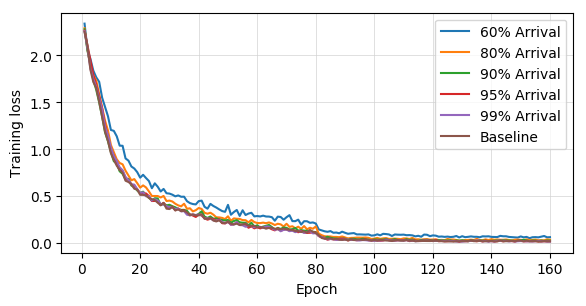
\includegraphics[width=0.4\textwidth,height=\textheight,keepaspectratio]{train_per_epoch_model_averaging_ResNet110}
%	}
%	\subfloat[Gradient Averaging]{
%		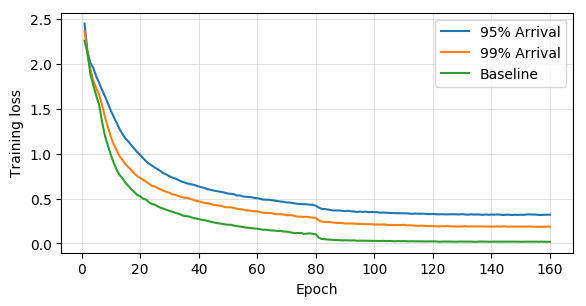
\includegraphics[width=0.4\textwidth,height=\textheight,keepaspectratio]{train_per_epoch_gradient_averaging_ResNet110}
%	}
%	\caption{Convergence of ResNet110 with CIFAR-10 on 16 GPUs.}
%	\label{fig:ResNet110}
%\end{figure*}
%
%\begin{figure*}[tbp]
%	\centering
%	\subfloat[Model Averaging]{
%		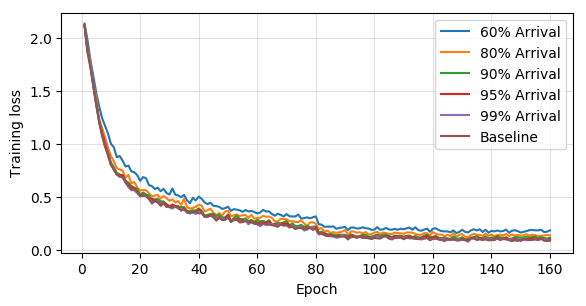
\includegraphics[width=0.4\textwidth,height=\textheight,keepaspectratio]{train_per_epoch_model_averaging_ResNet20}
%	}
%	\subfloat[Gradient Averaging]{
%		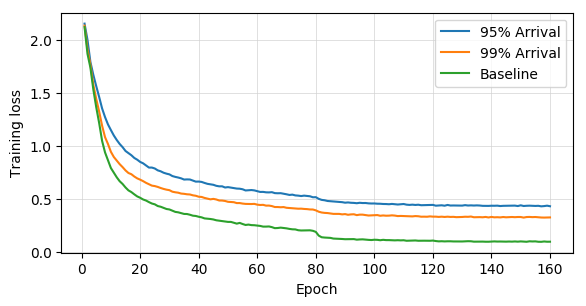
\includegraphics[width=0.4\textwidth,height=\textheight,keepaspectratio]{train_per_epoch_gradient_averaging_ResNet20}
%	}
%	\caption{Convergence of ResNet20 with CIFAR-10 on 16 GPUs.}
%	\label{fig:ResNet20}
%\end{figure*}


\begin{figure*}[tbp]
	\centering
	\subfloat[ResNet20 - CIFAR10]{
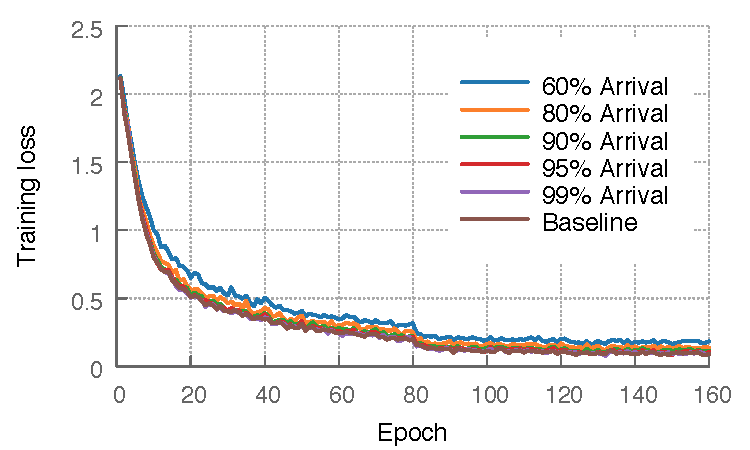
\includegraphics[width=0.33\textwidth,height=\textheight,keepaspectratio]{figures/plot_resnet20_model}
	}
	\subfloat[ResNet110 - CIFAR10]{
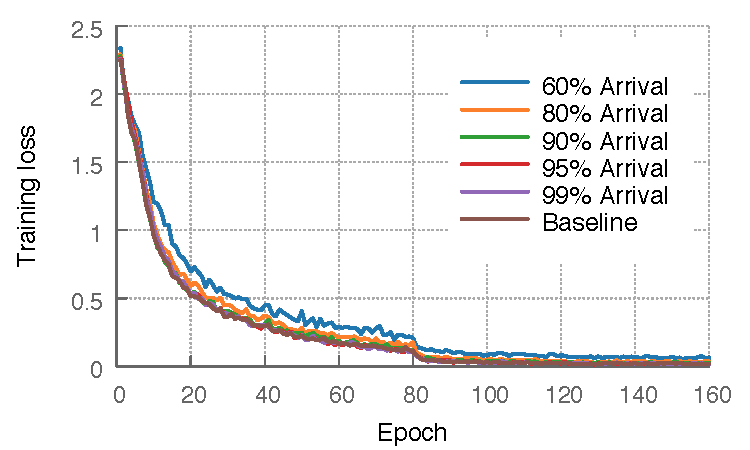
\includegraphics[width=0.33\textwidth,height=\textheight,keepaspectratio]{figures/plot_resnet110_model}
	}
	\subfloat[LSTM - ATIS]{
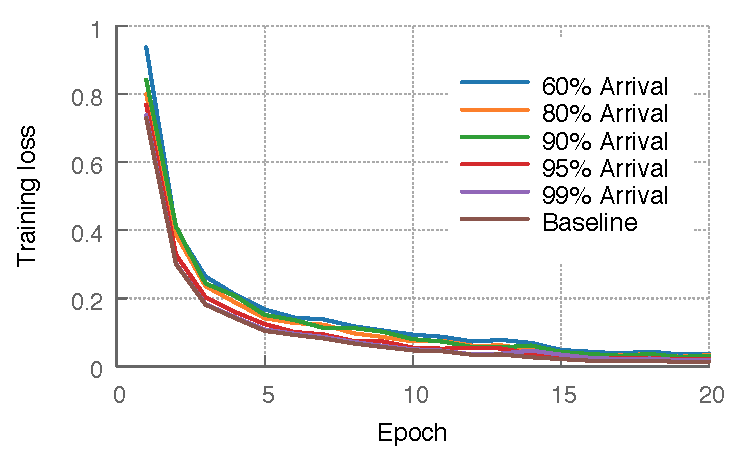
\includegraphics[width=0.33\textwidth,height=\textheight,keepaspectratio]{figures/plot_atis_model}
	}
    \caption{Convergence of RSAG on different datasets.}
    \label{fig:model}
\end{figure*}

\paragraph{Convergence of Image Classification} We perform convergence tests using the proven algorithm, model averaging SGD, on both ResNet110 and ResNet20 with CIFAR-10. Figure~\ref{fig:model}(a,b) shows
the result. We vary probabilities of a packet arriving at each node from 80\%, 90\%, 95\% and 99\%. The baseline is represented as a setting, where all the packages reached their recipient (100\%). The baseline achieves a training loss of 0.02 using ResNet110 and 0.09 for ResNet20. Dropping 1\% doesn't increase the training loss achieved after 160 epochs. For 5\% the training loss is identical on ResNet110 and increased by 0.02 on ResNet20. Having a probability of 90\% of arrival leads to a training loss of 0.03 for ResNet110 and 0.11 for ResNet20 respectively.

\paragraph{Convergence of NLU} We perform full convergence tests for the NLU task on the ATIS corpus and a single layer LSTM.
Figure~\ref{fig:model}(c) shows the result. The baseline achieves a training loss of 0.01. Dropping 1, 5 or 10 percent of the communicated partial vectors result in an increase of 0.01 in training loss.

%\begin{figure*}[tbp]
%	\centering
%	\subfloat[Model Averaging]{
%		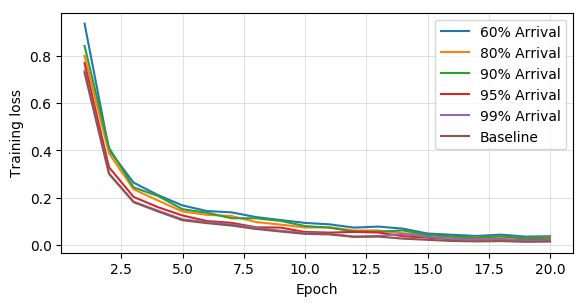
\includegraphics[width=0.4\textwidth,height=\textheight,keepaspectratio]{train_per_epoch_model_averaging_ATIS}
%	}
%	\subfloat[Gradient Averaging]{
%		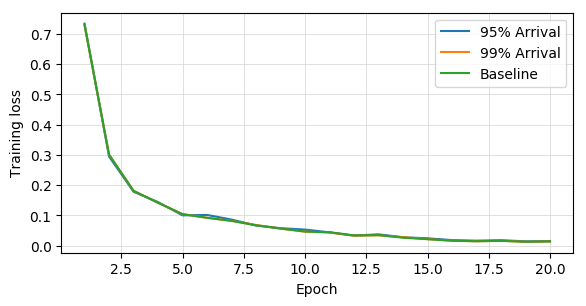
\includegraphics[width=0.4\textwidth,height=\textheight,keepaspectratio]{train_per_epoch_gradient_averaging_ATIS}
%	}
%	\caption{Convergence of LSTM network with ATIS on 8 GPUs.}
%	\label{fig:ATIS_LSTM}
%\end{figure*}

\begin{figure*}[tbp]
	\centering
	\subfloat[ResNet20 - CIFAR10]{
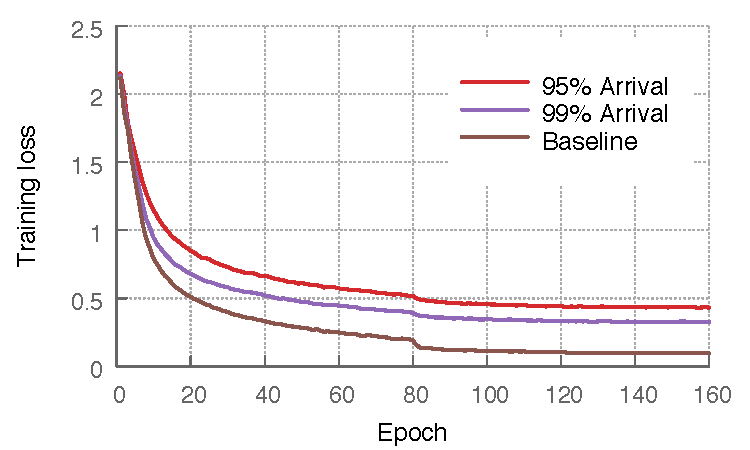
\includegraphics[width=0.33\textwidth,height=\textheight,keepaspectratio]{figures/plot_resnet20_gradient}
	}
	\subfloat[ResNet110 - CIFAR10]{
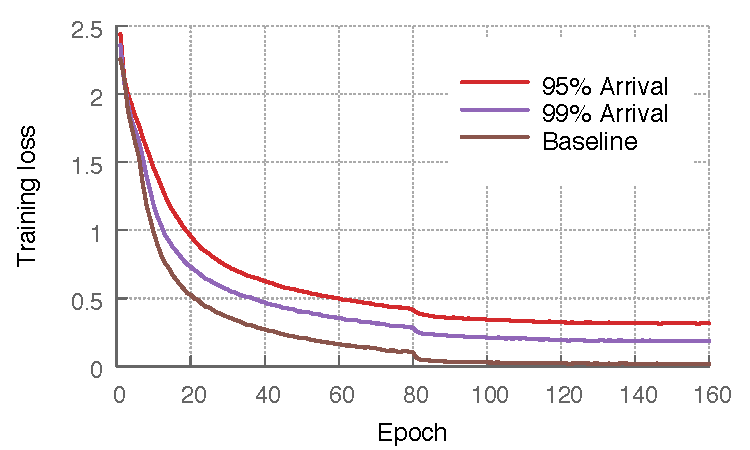
\includegraphics[width=0.33\textwidth,height=\textheight,keepaspectratio]{figures/plot_resnet110_gradient}
	}
	\subfloat[LSTM - ATIS]{
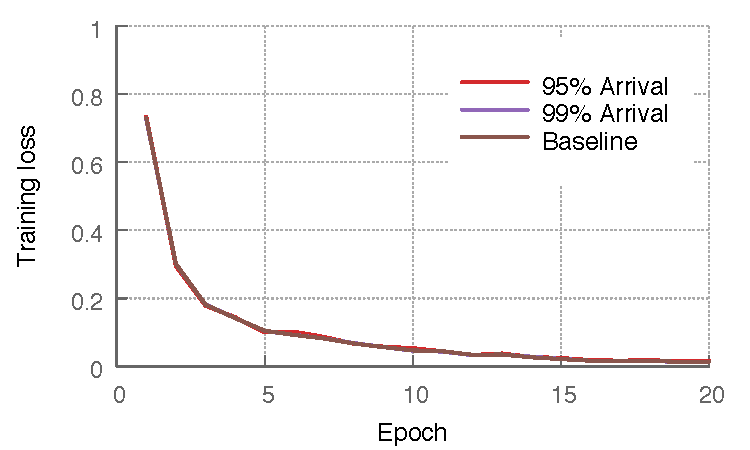
\includegraphics[width=0.33\textwidth,height=\textheight,keepaspectratio]{figures/plot_atis_gradient}
	}
    \caption{Why RSAG? The Behavior of Stanford AllReduce SGD in the Presence of Message Drop.}
    \label{fig:grad}
\end{figure*}

\paragraph{Why Model-averaging? Comparison with Gradient Averaging} We conduct experiments with identical setup and a probability of 99 percent of arrival using a gradient averaging methods instead of model averaging. When running data distributed SGD, gradient averaging is the most widely used technique in practice, also implemented by default in most deep learning frameworks\cite{abadi2016tensorflow, seide2016cntk}. As expected, the baseline (all the transmissions are successful) convergences to the same training loss as its model averaging counterpart, when omitting momentum and regularization terms. As seen in figures~\ref{fig:grad}(a,b), having a loss in communication of even 1 percentage results in worse convergence in terms of accuracy for both ResNet architectures on CIFAR-10. This behavior is not visible on the NLU examples. The reason for achieving similar training loss when dropping gradients randomly in this case lies most probably in the spars nature of the gradients and model given by the example. Dropping zero values communicated over the network does not affect convergence obviously. Nevertheless, this insight suggest that one should favor a model averaging algorithm over gradient averaging, if the underlying network connection is unreliable.

% \vspace{-0.5em}
\section{Case study: Speeding up Colocated Applications}
% \vspace{-1em}

\begin{figure}[h]
\centering
\begin{minipage}{.3\textwidth}
  \centering
  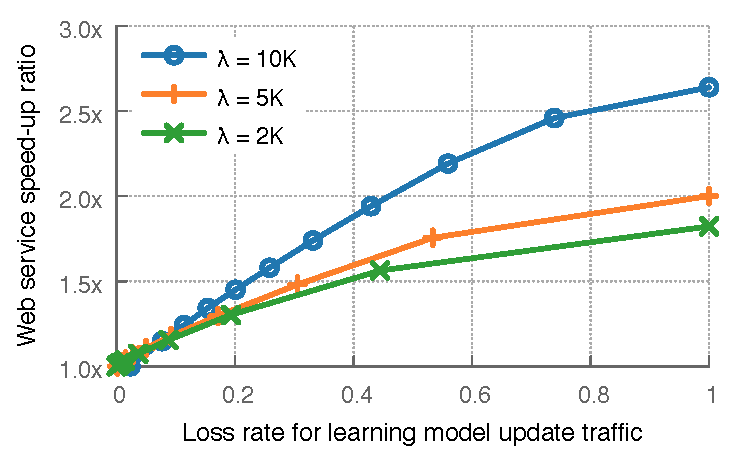
\includegraphics[width=1.0\linewidth]{ml_drop_rate_to_speed_up}%[width=1.0\linewidth]
  \captionof{figure}{Allowing an increasing rate of losses for model updates speeds up the Web service.}
  \label{fig:drop-rate-to-speed-up}
\end{minipage}%
\hspace{0.05\textwidth}%
\begin{minipage}{.3\textwidth}
  \centering
  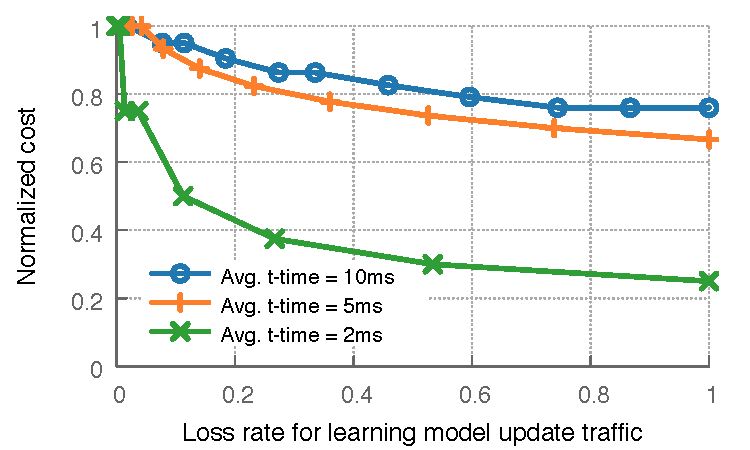
\includegraphics[width=1.0\linewidth]{ml_drop_rate_to_normalized_cost}%[width=1.0\linewidth]
  \captionof{figure}{Allowing more losses for model updates reduces the cost for the Web service.}
  \label{fig:drop-rate-to-normalized-cost}
\end{minipage}%
\end{figure}

Our results on the resilience of distributed learning to losses of model updates open up an interesting use case. That model updates can be lost (within some tolerance) without the deterioration of model convergence implies that model updates transmitted over the physical network can be de-prioritized compared to other more ``inflexible'' traffic, such as for Web services. Thus, we can colocate other applications with the training workloads, and reduce infrastructure costs for running them. Equivalently, workloads that are colocated with learning workers can benefit from prioritized network traffic (at the expense of some model update losses), and thus achieve lower latency.

%Neural networks have become so large that it has become unfeasible to train them on a single node. As such, the training is distributed over many nodes. These nodes are connected via a network, over which the model updates are sent. Up until now, the model updates have been sent reliably, which means that every packet must arrive before proceeding. However, as made evident in this work, it is not necessary for all of these updates to arrive to converge as well. We can make use of this insight by instead of sending model update flows over the network \textit{reliably}, we send them \textit{unreliably}. From a network perspective the benefit comes from the fact that the traffic of the machine learning workload can be partially dropped in times of congestion, freeing up network capacity to better serve other workloads active on the cluster.

To demonstrate this in practice, we perform a packet simulation over 16 servers, each connected with a $1$~Gbps link to a network switch. 
%As such, the network has a bisection bandwidth of 16 Gbps. 
Over this network of $16$ servers, we run two workloads: (a) replaying traces from the machine learning process of ResNet110 on CIFAR-10 (which translates to a load of 2.4 Gbps) which is sent \emph{unreliably}, and (b) a simple emulated Web service running on all $16$ servers. Web services often produce significant background traffic between servers within the data center, consisting typically of small messages fetching distributed pieces of content to compose a response (i.e. a Google query response potentially consists of advertisements, search results, and images). We emulate this intra data center traffic for the Web service as all-to-all traffic between these servers, with small messages of $100$~KB (a reasonable size for such services) sent reliably between these servers. The inter-arrival time for these messages follows a Poisson process, parametrized by the expected message rate, $\lambda$ (aggregated across the $16$ servers).  

Different degrees of prioritization of the Web service traffic over learning traffic result in different degrees of loss in learning updates transmitted over the network. As the Web service is prioritized to a greater extent, its performance improves -- its message exchanges take less time; we refer to this reduction in (average) completion time for these messages as a speed-up. Note that even small speedups of $10\%$ are significant for such services; for example, Google actively pursues minimizing its Web services' response latency. An alternative method of quantifying the benefit for the colocated Web service is to measure how many additional messages the Web service can send, while maintaining a fixed average completion time. This translates to running more Web service queries and achieving more throughput over the same infrastructure, thus reducing cost per request / message.

%We model how much the network prioritizes the background traffic by introducing a buffer threshold: every time a ML packet arrives at a buffer queue it is inserted iff the resulting buffer free room is more than the threshold.

%By increasing the fraction of ML flow that can be dropped, network capacity is vacated for the background traffic. The effect of this we demonstrate in two ways. First, by keeping the flow arrival rate fixed, we measure how much the average flow completion (FCT) of the web service improves as we increase the fraction of ML flow dropped. This speed-up ratio improvement is shown in Fig. \ref{fig:drop-rate-to-speed-up}. The amount a larger fraction of the machine learning flows is dropped because it has to compete with more background flows. Increasingly unreliable transmission 

Fig.~\ref{fig:drop-rate-to-speed-up} and \ref{fig:drop-rate-to-normalized-cost} show results for the above described Web service speedup and cost reduction respectively. In Fig.~\ref{fig:drop-rate-to-speed-up}, the arrival rate of Web service messages is fixed ($\lambda = \{2000, 5000, 10000\}$ per second). As the network prioritizes the Web service more and more over learning update traffic, more learning traffic suffers losses (on the $x$-axis), but performance for the Web service improves. With just $10\%$ losses for learning updates, the Web service can be sped up by more than $20\%$ (\emph{i.e.,} $1.2\times$). 

In Fig.~\ref{fig:drop-rate-to-normalized-cost}, we set a target average transmission time ($2$, $5$, or $10$~ms) for the Web service's messages, and increase the message arrival rate, $\lambda$, thus causing more and more losses for learning updates on the $x$-axis. But accommodating higher $\lambda$ over the same infrastructure translates to a lower cost of running the Web service (with this reduction shown on the $y$-axis).

Thus, tolerating small amounts of loss in model update traffic can result in significant benefits for colocated services, while not deteriorating model convergence.

% \vspace{-0.5em}
\section{Conclusion}
% \vspace{-1em}

We present a novel decentralized learning algorithm
RSAG, which models a realistic scenario of distributed learning
over unreliable networks. Mathemat
ically, RSAG is the same
as decentralized, distributed learning over randomized topology.
We present a novel theoretical analysis for such scenario and
evaluate it with training neural networks on both image and natural language datasets. We also provide a case study of application 
collocation to illustrate the potential benefit that can be provided
by allowing learning algorithms to take advantage of 
unreliable communication channels.


%Because the network capacity is fixed and flows continue to arrive relentlessly at a fixed arrival rate, at some load point the network becomes congested. The more background traffic is prioritized by increasing \textit{Buff-T}, at a lower arrival rate an equal amount of ML flow is dropped. We show the relative gain over reliable transmission by unreliably transmitting instead in various network prioritization cases. The unreliable congestion control mechanism of the ML flows is more aggressive than its reliable counterpart, resulting in the < 1 normalized throughput at $\text{Buff-T}=0$, when the ML packets compete equally (0.4\% ML flow drop rate). At $\text{Buff-T}=1$, all the ML packets are dropped (100\% ML flow drop rate). At $\text{Buff-T}=0.3$ an additional 20\% background traffic is sustained, while suffering a 10\% drop of ML flow. The increasing trend of web service speed-up in Fig. \ref{fig:drop-rate-to-speed-up} and the decreasing normalized cost at equal performance in Fig. \ref{fig:drop-rate-to-normalized-cost} shows that there is possible gain in the unreliable sending of machine learning traffic, though highlights the need for a mechanism to ensure that not too much of the ML flow is dropped should be in place.

%To further this innovation, we identify the following three tasks that lay ahead in future work. (1) We want to investigate the relation between the beneficial time effect of model update flows finishing earlier and the additional convergence time it incurs by the decrease in information it causes. (2) We want to explore (new) network techniques (i.e. congestion control schemes, prioritization) that can be applied best to fairly balance the background and machine learning workload. (3) We want to evaluate the performance gain using a wider range of workloads, and networks, particularly when the background traffic is bursty. When pushed to its fullest extent, we believe this application can lead to the ambitious implementation of an unreliable-transmission machine learning framework which enables higher performance of co-located workloads than when using traditional reliable-transmission frameworks while still achieving equally good machine learning application-layer performance.

%In this small-scale demonstration, by making use of unreliable transmission, we have gained the ability to support \todo{QUA}\% more background flows, shown in Fig. \ref{fig:network_application} as the distance between the two horizontal lines. This small-scale demonstration is a first indication of the potential gain unreliable sending of machine learning traffic can achieve



%\begin{figure}
%  \centering
%  \includegraphics[width=0.5\linewidth]{ml_drop_rate_to_bg_arrival_rate.pdf}
%  \caption{Other ("background") traffic can be better serviced simultaneously with the machine learning workload when applying the technique.}
%  \label{fig:network_application}
%\end{figure}

\clearpage

%\subsubsection*{Acknowledgments}

\bibliography{references}
\bibliographystyle{plain}

\newpage
\appendix

\begin{center}
{\Huge \bf
Supplemental Materials
}
\end{center}

\section {Notations}
In order to unify notations, we define the following notations about gradient:
\begin{align*}
\bm{g}^{(i)}(\bm{x}^{(i)}_t;\bm{\xi}^{(i)}_t) = \nabla F_i(\bm{x}^{(i)}_t;\bm{\xi}^{(i)}_t)
\end{align*}
\subsection{Matrix Notations}
We aggregate vectors into matrix, and using matrix to simplify the proof.
\begin{align*}
	X_t &:= \left(\bm{x}_t^{(1)}, \bm{x}_t^{(2)}, \cdots, \bm{x}_t^{(n)}\right)\\
	V_t &:= \left(\bm{v}_t^{(1)}, \bm{v}_t^{(2)}, \cdots, \bm{v}_t^{(n)}\right)\\
	\Xi_t &:= \big(\bm{\xi}_t^{(1)}, \bm{\xi}_t^{(2)}, \cdots, \bm{\xi}_t^{(n)}\big)\\
	G(X_t;\Xi_t)&:= \left(\bm{g}^{(1)}(\bm{x}_t^{(1)};\bm{\xi}_t^{(1)}),\cdots,\bm{g}^{(n)}(\bm{x}_t^{(n)};\bm{\xi}_t^{(n)}) \right)
\end{align*}

\subsection{Averaged Notations}
We define averaged vectors as follows:
\begin{align*}
	\overline{\bm{x}}_t &:= X_t\frac{\mathbf{1}}{n} \numberthis\label{re: 1}\\
	\overline{\bm{v}}_t &:= V_t\frac{\mathbf{1}}{n} \numberthis\label{re: 7}\\
	\overline{\bm{g}}(X_t;\Xi_t) &:= G(X_t;\Xi_t)\frac{\mathbf{1}}{n} \numberthis\label{re: 8}\\
	\overline{\nabla}f(X_t)&:= \frac{1}{n}\sum\limits_{i=1}^n f_i(\bm{x}_t^{(i)})\\
	\Delta \overline{\bm{x}}_t &:= \overline{\bm{x}}_{t+1} - \overline{\bm{x}}_t
\end{align*}

\subsection{Block Notations}
Remember in (\ref{eq: dividev}) and (\ref{eq: dividex}), we have divided models in blocks:
\begin{align*}
\bm{v}_t^{(i)} = &\left(\left(\bm{v}_t^{(i,1)}\right)^{\top}, \left(\bm{v}_t^{(i,2)}\right)^{\top}, \cdots, \left(\bm{v}_t^{(i,n)}\right)^{\top}\right)^{\top}\\
\bm{x}_{t}^{(i)} = &\left(\left(\bm{x}_{t}^{(i,1)}\right)^{\top}, \left(\bm{x}_{t}^{(i,2)}\right)^{\top},\cdots, \left(\bm{x}_{t}^{(i,n)}\right)^{\top}\right)^{\top}, \forall i\in[n].
\end{align*}
 We do the some division on some other quantities, see following (the dimension of each block is the same as the corresponding block in $\bm{v}_t^{(i)}$) : 
\begin{align*}
	\overline{\bm{x}}_t &= \left(\left(\overline{\bm{x}}_t^{(1)}\right)^{\top},\left(\overline{\bm{x}}_t^{(2)}\right)^{\top},\cdots, \left(\overline{\bm{x}}_t^{(n)}\right)^{\top}\right)^{\top}\\
	\overline{\bm{v}}_t &= \left(\left(\overline{\bm{v}}_t^{(1)}\right)^{\top},\left(\overline{\bm{v}}_t^{(2)}\right)^{\top},\cdots, \left(\overline{\bm{v}}_t^{(n)}\right)^{\top}\right)^{\top}\\
	\Delta \overline{\bm{x}}_t &= \left(\left(\Delta^{(1)} \overline{\bm{x}}_t\right)^{\top}, \left(\Delta_t^{(2)} \overline{\bm{x}}\right)^{\top}, \cdots, \left(\Delta_t^{(n)} \overline{\bm{x}}\right)^{\top}\right)^{\top}\\
	\bm{g}^{(i)}(\cdot; \cdot) &= \left(\left(\bm{g}^{(i,1)}(\cdot; \cdot)\right)^{\top}, \left(\bm{g}^{(i,2)}(\cdot; \cdot)\right)^{\top}, \cdots, \left(\bm{g}^{(i,n)}(\cdot; \cdot)\right)^{\top}\right)^{\top}\\
	\overline{\bm{g}}(X_t;\Xi_t) &= \left(\left(\overline{\bm{g}}^{(1)}(X_t;\Xi_t)\right)^{\top},\cdots, \left(\overline{\bm{g}}^{(n)}(X_t;\Xi_t)\right)^{\top}\right)^{\top}\\
	\nabla f_i(\bm{x}_t^{(i)}) &= \left(\left(\nabla^{(1)} f_i(\bm{x}_t^{(i)})\right)^{\top}, \left(\nabla^{(2)} f_i(\bm{x}_t^{(i)})\right)^{\top}, \cdots, \left(\nabla^{(n)} f_i(\bm{x}_t^{(i)})\right)^{\top}\right)^{\top}\\
	\overline{\nabla} f(X_t) &= \left(\left(\overline{\nabla}^{(1)} f(X_t)\right)^{\top}, \left(\overline{\nabla}^{(2)} f(X_t)\right)^{\top}, \cdots, \left(\overline{\nabla}^{(n)} f(X_t)\right)^{\top}\right)^{\top}\\
	\nabla f(\overline{\bm{x}}_t)&= \left(\left(\nabla^{(1)} f(\overline{\bm{x}}_t)\right)^{\top}, \left(\nabla^{(2)} f(\overline{\bm{x}}_t)\right)^{\top}, \cdots, \left(\nabla^{(n)} f(\overline{\bm{x}}_t)\right)^{\top}\right)^{\top}.
\end{align*}

\subsection{Aggregated Block Notations}
Now, we can define some additional notations throughout the following proof
\begin{align*}
X_t^{(j)}:=&(\bm{x}_t^{(1,j)},\bm{x}_t^{(2,j)},\cdots,\bm{x}_t^{(n,j)})\\
V_t^{(j)}:=&(\bm{v}_t^{(1,j)},\bm{v}_t^{(2,j)},\cdots,\bm{v}_t^{(n,j)})\\
G^{(j)}(X_t;\Xi_t):= &\left(\bm{g}^{(1,j)}(\bm{x}_t^{(1)};\bm{\xi}_t^{(1)}),\cdots,\bm{g}^{(n,j)}(\bm{x}_t^{(n)};\bm{\xi}_t^{(n)}) \right)
\end{align*}

\subsection{Relations between Notations}
We have the following relations between these notations:
\begin{align*}
	\overline{\bm{x}}_t^{(j)} &= X_t^{(j)}\frac{\mathbf{1}}{n} \numberthis\label{re: 2}\\
	\overline{\bm{v}}_t^{(j)} &= V_t^{(j)}\frac{\mathbf{1}}{n} \numberthis\label{re: 3}\\
	\overline{\bm{g}}^{(j)}(X_t;\Xi_t) &= G^{(j)}(X_t;\Xi_t)\frac{\mathbf{1}}{n} \numberthis\label{re: 9}\\
	A_nA_n &= A_n \numberthis\label{re: 4}\\ 
	V_t &= X_t - \gamma G(X_t; \Xi_t) \numberthis\label{re: 5}\\
	V_t^{(j)} &= X_t^{(j)} - \gamma G^{(j)}(X_t; \Xi_t) \numberthis\label{re: 6}
\end{align*}

\subsection{Expectation Notations}
There are different conditions when taking expectations in the proof, so we list these conditions below:
\paragraph{$\mathbb{E}_{t,G}[\cdot]$}
Denote taking the expectation over the \textbf{computing stochastic Gradient} procedure at $t$th iteration on condition of the history information before the $t$th iteration.
\paragraph{$\mathbb{E}_{t,P}[\cdot]$}
Denote taking the expectation over the \textbf{Package drop in sending and receiving blocks} procedure at $t$th iteration on condition of the history information before the $t$th iteration and the SGD procedure at the $t$th iteration.
\paragraph{$\mathbb{E}_t[\cdot]$}
Denote taking the expectation over all procedure during the $t$th iteration on condition of the history information before the $t$th iteration.
\paragraph{$\mathbb{E}[\cdot]$}
Denote taking the expectation over all history information.

\subsection{Others}
We define $I_n$ as the $n\times n$ identity matrix, $\mathbf{1}_n$ as $(1,1,\cdots, 1)^\top$ and $A_n$ as $\frac{1}{n}\mathbf{1}\mathbf{1}^{\top}$. Also, we suppose the packet drop rate is $p$.

The following equation is used frequently:
\begin{equation} \label{eq: T}
	\Tr (XA_nX^{\top}) = \Tr\Big(X\frac{\mathbf{1}\mathbf{1}^{\top}}{n}X^{\top}\Big) = n\Tr \bigg(\Big( X\frac{\mathbf{1}}{n}\Big)^{\top}X\frac{\mathbf{1}}{n}\bigg) = n\Big( X\frac{\mathbf{1}}{n}\Big)^{\top}X\frac{\mathbf{1}}{n} = n\left\|X\frac{\mathbf{1}}{n}\right\|^2
\end{equation}









\section{Proof to Theorem~\ref{theo:1}}
The critical part for a decentralized algorithm to be successful, is that local model on each node will converge to their average model. We summarize this critical property by the next lemma.

\begin{lemma}\label{L:xavekey}
From the updating rule (\ref{eq: updatingrule}) and Assumption \ref{ass:global}, we have
\begin{align*}
\sum_{s=1}^T\sum_{i=1}^n\mathbb E\left\|\bm{x}_{s+1}^{(i)} - \overline{\bm{x}}_{s+1}\right\|^2 \leq & \frac{2\gamma^2n\sigma^2TC_1}{(1-\sqrt{\beta})^2} + \frac{6n\zeta^2TC_1}{(1-\sqrt{\beta})^2},\numberthis\label{lemma:xavekey}
\end{align*}
where $C_1:=\left(1- \frac{6L^2\gamma^2}{(1-\sqrt{\beta})^2} \right)^{-1}$ and $\beta = \alpha_2 - \alpha_3 $.
\end{lemma}

We will prove this critical property first. Then, after proving some lemmas, we will prove the final theorem. During the proof, we will use properties of weighted matrix $W_t^{(j)}$ which is showed in \textbf{Section ~\ref{secD}}.

\subsection{Proof of Lemma~\ref{L:xavekey}} 
\begin{proof} [\textbf{Proof to Lemma~\ref{L:xavekey}}]
According to updating rule (\ref{eq: updatingrule}) and Assumption \ref{ass:global}, we have
\begin{align*}
X_{t+1}^{(j)} = & V_t^{(j)}W_{t}^{(j)}\\
= & \left(X_t^{(j)} - \gamma G^{(j)}(X_t;\Xi_t)\right)W_{t}^{(j)}\\
= & X_1^{(j)}\prod_{r=1}^t W_{r}^{(j)} - \gamma\sum_{s=1}^tG^{(j)}(X_s;\Xi_s)\prod_{r=s}^tW_{r}^{(j)}\\
= & - \gamma\sum_{s=1}^tG^{(j)}(X_s;\Xi_s)\prod_{r=s}^tW_{r}^{(j)}. \text{   } \left(\text{due to } X_1 = 0\right)\numberthis\label{lemma:xavekey_1} 
\end{align*}

We also have 
\begin{align*}
\sum_{i=1}^n\left\|\bm{x}_{t+1}^{(i,j)} - \overline{\bm{x}}_{t+1}^{(j)}\right\|^2 = &\left\|X_{t+1}^{(j)} - X_{t+1}^{(j)}\frac{\bm{1}}{n}\bm{1}^{\top}_n \right\|^2_F =  \left\|X_{t+1}^{(j)} - X_{t+1}^{(j)}A_n \right\|^2_F \numberthis\label{lemma:xavekey_2}
\end{align*}
Combing \eqref{lemma:xavekey_1} and \eqref{lemma:xavekey_2} together, and define
\begin{align*}
H_{t,s}^{(j)} : = G^{(j)}(X_s;\Xi_s)\prod_{r=s}^tW_{r}^{(j)}
\end{align*}
we get
\begin{align*}
\sum_{i=1}^n\left\|\left(\bm{x}_{t+1}^{(i,j)} - \overline{\bm{x}}_{t+1}^{(j)}\right)\right\|^2 = & \left\|X_{t+1}^{(j)}(I_n - A_n) \right\|^2_F\\
= & \gamma^2\left\|\sum_{s=1}^tH_{t,s}^{(j)}(I_n-A_n) \right\|^2_F\\
= & \gamma^2 \Tr\left((I_n-A_n)\sum_{s=1}^t\left(H_{t,s}^{(j)}\right)^{\top}\sum_{s'=1}^tH_{t,s'}^{(j)}(I-An) \right)\\
= & \gamma^2 \sum_{s,s'=1}^t\Tr\left((I_n-A_n)\left(H_{t,s}^{(j)}\right)^{\top}H_{t,s'}^{(j)}(I-An) \right)\\
\leq & \frac{\gamma^2}{2} \sum_{s,s'=1}^t\left( k_{s,s'}\left\|H_{t,s}^{(j)}(I_n-A_n)\right\|^2_F + \frac{1}{k_{s,s'}}\left\|H_{t,s'}^{(j)}(I_n-A_n)\right\|^2_F \right) ,\numberthis\label{lemma:xavekey_3}
\end{align*}
where $k_{s,s'}$ is a scale factor that is to be computed later. The last inequality is because $2\Tr(A^{\top}B)\leq k\|A\|_F^2 + \frac{1}{k}\|B\|_F^2$ for any matrix $A$ and $B$.

For $\left\|H_{t,s}^{(j)}(I_n-A_n)\right\|^2_F$, we have
\begin{align*}
&\mathbb E \left\|H_{t,s}^{(j)}(I_n-A_n)\right\|^2_F\\
 = & \mathbb E\Tr\left( G^{(j)}(X_s;\Xi_s)W_{s}^{(j)}\cdots W_{t}^{(j)} (I_n-A_n) \left(W_{t}^{(j)}\right)^{\top}\cdots  \left(W_{s}^{(j)}\right)^{\top} \left(G^{(j)}(X_s;\Xi_s)\right)^{\top}  \right). \numberthis\label{lemma: keyyc_1}
\end{align*}

Now we can take expectation from time $t-1$ back to time $s-1$. When taking expectation of time $t$, we only need to compute $\mathbb{E} \left[W_t^{(j)}(I_n-A_n)\left(W_t^{(j)}\right)^{\top}\right]$. From Lemma \ref{lem: EWW} and Lemma \ref{lem: EWAW}, this is just $(\alpha_2 - \alpha_3)(I_n-A_n)$. Applying this to (\ref{lemma: keyyc_1}), we can get the similar form except replacing $t$ by $t-1$ and multiplying by factor $\alpha_2-\alpha_3$. Therefore, we have the following:
\begin{align*}
\mathbb E \left\|H_{t,s}^{(j)}(I_n-A_n)\right\|^2_F = & (\alpha_2- \alpha_3)^{t-s+1}\mathbb{E} \left\|G^{(j)}(X_s;\Xi_s)(I_n-A_n)\right\|^2_F\\
 \leq & (\alpha_2-\alpha_3)^{t-s}\mathbb{E} \left\|G^{(j)}(X_s;\Xi_s)(I_n-A_n)\right\|^2_F.
\end{align*}
The last inequality comes from $\alpha_3\le \alpha_2$c and $\beta = \alpha_2-\alpha_3 $ is defined in Theorem~\ref{theo:1} .

Then \eqref{lemma:xavekey_3} becomes
\begin{align*}
&\sum_{i=1}^n\left\|\left(\bm{x}_{t+1}^{(i,j)} - \overline{\bm{x}}_{t+1}^{(j)}\right)\right\|^2\\
 \leq  & \frac{\gamma^2}{2} \sum_{s,s'=1}^t\left( k_{s,s'}\beta^{t-s}\left\|G^{(j)}(X_s;\Xi_s)(I_n-A_n)\right\|^2_F + \frac{1}{k_{s,s'}}\beta^{t-s'}\left\|G^{(j)}(X_{s'};\xi_{s'})(I_n-A_n)\right\|^2_F \right).
\end{align*}
So if we choose $k_{s,s'} = \beta^{\frac{s-s'}{2}}$, the above inequality becomes
\begin{align*}
&\sum_{i=1}^n\left\|\left(\bm{x}_{t+1}^{(i,j)} - \overline{\bm{x}}_{t+1}^{(j)}\right)\right\|^2\\
 \leq  & \frac{\gamma^2}{2} \sum_{s,s'=1}^t\left( \beta^{\frac{2t-s-s'}{2}}\left\|G^{(j)}(X_s;\Xi_s)(I_n-A_n)\right\|^2_F + \beta^{\frac{2t-s'-s}{2}}\left\|G^{(j)}(X_{s'};\xi_{s'})(I_n-A_n)\right\|^2_F \right)\\
 = & \frac{\gamma^2\beta^{t}}{2} \sum_{s,s'=1}^t\beta^{\frac{-s-s'}{2}}\left( \left\|G^{(j)}(X_s;\Xi_s)(I_n-A_n)\right\|^2_F + \left\|G^{(j)}(X_{s'};\xi_{s'})(I_n-A_n)\right\|^2_F \right)\\
 = & \gamma^2\beta^{t} \sum_{s,s'=1}^t\beta^{\frac{-s-s'}{2}} \left\|G^{(j)}(X_s;\Xi_s)(I_n-A_n)\right\|^2_F \\
 = & \gamma^2 \sum_{s=1}^t\beta^{\frac{t-s}{2}} \left\|G^{(j)}(X_s;\Xi_s)(I_n-A_n)\right\|^2_F \sum_{s'=1}^t \beta^{\frac{t-s'}{2}}\\
 \leq & \frac{\gamma^2}{1-\sqrt{\beta}} \sum_{s=1}^t\beta^{\frac{t-s}{2}} \left\|G^{(j)}(X_s;\Xi_s)(I_n-A_n)\right\|^2_F \numberthis\label{lemma:xavekey_4}
\end{align*}


We also have: 
\begin{align*}
&\sum_{j=1}^n\mathbb E\left\|G^{(j)}(X_s;\Xi_s)(I_n-A_n)\right\|_F^2\\
=& \sum_{j=1}^n\sum_{i=1}^n\mathbb E_{t,G}\left\|\bm{g}^{(i,j)}(\bm{x}_t^{(i)};\bm{\xi}_t^{(i)}) - \overline{\bm{g}}^{(j)}(X_t;\Xi_t)\right\|^2\\
\leq & \sum_{j=1}^n\sum_{i=1}^n\mathbb E_{t,G}\left\|\bm{g}^{(i,j)}(\bm{x}_t^{(i)};\bm{\xi}_t^{(i)}) -\nabla^{(j)} f_i(\bm{x}_t^{(i)})\right\|^2 \\
& + 3\sum_{j=1}^n\sum_{i=1}^n\left\| \nabla^{(j)} f_i(\overline{\bm{x}}_t) - \nabla^{(j)} f(\overline{\bm{x}}_t) \right\|^2 + 6L\sum_{j=1}^n\sum_{i=1}^n\left\|\bm{x}_t^{(i,j)} - \overline{\bm{x}}_t^{(j)}\right\|^2 \text{    } (\text{using } \eqref{lemma:key_4})\\
= & \sum_{i=1}^n\mathbb E_{t,G}\left\|\bm{g}^{(i)}(\bm{x}_t^{(i)};\bm{\xi}_t^{(i)}) -\nabla f^{(i)}(\bm{x}_t^{(i)})\right\|^2 \\
& + 3\sum_{i=1}^n\left\| \nabla f^{(i)}(\overline{\bm{x}}_t) - \nabla f(\overline{\bm{x}}_t) \right\|^2 + 6L\sum_{i=1}^n\left\|\bm{x}_t^{(i)} - \overline{\bm{x}}_t\right\|^2\\
\leq & n\sigma^2 + 6L\sum_{i=1}^n\left\|\overline{\bm{x}}_s - \bm{x}_s^{(i)}\right\|^2 + 3n\zeta^2 
\end{align*}

From the inequality above and \eqref{lemma:xavekey_4} we have
\begin{align*}
&\sum_{j=1}^n\sum_{s=1}^T\sum_{i=1}^n\mathbb E\left\|\bm{x}_{s+1}^{(i,j)} - \overline{\bm{x}}_{s+1}^{(j)}\right\|^2 \\
\leq & \left(\frac{\gamma^2n\sigma^2}{1-\sqrt{\beta}} + \sum_{j=1}^n\frac{3n\zeta^2}{1-\sqrt{\beta}}\right)\sum_{s=1}^T\sum_{r=1}^s\beta^{\frac{s-r}{2}} + \frac{6L^2\gamma^2}{1-\sqrt{\beta}}\sum_{s=1}^T\sum_{r=1}^s\sum_{i=1}^n\beta^{\frac{s-r}{2}}\left\|\overline{\bm{x}}_r- \bm{x}_r^{(i)}\right\|^2\\
\leq & \frac{\gamma^2n\sigma^2T}{(1-\sqrt{\beta})^2} + \frac{n\zeta^2T}{(1-\sqrt{\beta})^2} + \frac{6L^2\gamma^2}{1-\sqrt{\beta}}\sum_{i=1}^n\sum_{s=1}^T\sum_{r=1}^s\beta^{\frac{s-r}{2}}\left\|\overline{\bm{x}}_r- \bm{x}_r^{(i)}\right\|^2\\
= & \frac{\gamma^2n\sigma^2T}{(1-\sqrt{\beta})^2} + \frac{3n\zeta^2T}{(1-\sqrt{\beta})^2} + \frac{6L^2\gamma^2}{1-\sqrt{\beta}}\sum_{i=1}^n\sum_{r=1}^T\sum_{s=r}^T\beta^{\frac{s-r}{2}}\left\|\overline{\bm{x}}_r- \bm{x}_r^{(i)}\right\|^2\\
= & \frac{\gamma^2n\sigma^2T}{(1-\sqrt{\beta})^2} + \frac{3n\zeta^2T}{(1-\sqrt{\beta})^2} + \frac{6L^2\gamma^2}{1-\sqrt{\beta}}\sum_{i=1}^n\sum_{r=1}^T\sum_{s=0}^{T-r}\beta^{\frac{s}{2}}\left\|\overline{\bm{x}}_r- \bm{x}_r^{(i)}\right\|^2\\
\leq  & \frac{\gamma^2n\sigma^2T}{(1-\sqrt{\beta})^2} + \frac{3n\zeta^2T}{(1-\sqrt{\beta})^2} + \frac{6L^2\gamma^2}{(1-\sqrt{\beta})^2}\sum_{i=1}^n\sum_{r=1}^T\left\|\overline{\bm{x}}_r- \bm{x}_r^{(i)}\right\|^2.
\end{align*}
If $\gamma$ is small enough that satisfies $\left(1- \frac{6L^2\gamma^2}{(1-\sqrt{\beta})^2} \right) > 0$, then we have
\begin{align*}
\left(1- \frac{6L^2\gamma^2}{(1-\sqrt{\beta})^2} \right) \sum_{s=1}^T\sum_{i=1}^n\mathbb E\left\|\bm{x}_{s}^{(i)} - \overline{\bm{x}}_{s}\right\|^2 \leq & \frac{\gamma^2n\sigma^2T}{(1-\sqrt{\beta})^2} + \frac{3n\zeta^2T}{(1-\sqrt{\beta})^2}.
\end{align*}
Denote $C_1:=\left(1- \frac{6L^2\gamma^2}{(1-\sqrt{\beta})^2} \right)^{-1}$, then we have
\begin{align*}
\sum_{s=1}^T\sum_{i=1}^n\mathbb E\left\|\bm{x}_{s}^{(i)} - \overline{\bm{x}}_{s}\right\|^2 \leq & \frac{2\gamma^2n\sigma^2TC_1}{(1-\sqrt{\beta})^2} + \frac{6n\zeta^2TC_1}{(1-\sqrt{\beta})^2}.
\end{align*}

\end{proof}



\subsection{Proof to Theorem~\ref{theo:1}}


\begin{lemma}\label{L:deltax}
From the updating rule (\ref{eq: updatingrule}) and Assumption \ref{ass:global}, we have
\begin{align*}
\mathbb{E}_{t,P}\big[\left\|\Delta\overline{\bm{x}}_t\right\|^2\big] = &\frac{\alpha_3}{n}\sum_{j=1}^n \Tr\left( \left(V_t^{(j)}\right)^{\top}\left(I_n-A_n\right)V_t^{(j)} \right) +  \gamma^2 \left\| \overline{\bm{g}}(X_t;\Xi_t) \right\|^2,\\
\mathbb{E}_{t,P}[\Delta\overline{\bm{x}}_t]= &-\gamma \overline{\bm{g}}(X_t; \Xi_t).
\end{align*}
\begin{proof}
We begin with $\mathbb{E}_{t,P}\big[\left\|\Delta\overline{\bm{x}}_t\right\|^2\big]$: 
\begin{align*}
\mathbb{E}_{t,P}\big[\left\|\Delta\overline{\bm{x}}_t\right\|^2\big] =&  \sum\limits_{j=1}^n \mathbb{E}_{t,P}\Big[\left\|\Delta^{(j)}\overline{\bm{x}}_t\right\|^2\Big]\\
\xlongequal{(\ref{re: 2})}& \sum_{j=1}^n\mathbb{E}_{t,P}\bigg[\left\| \left(X_{t+1}^{(j)} - X_{t}^{(j)}\right)\frac{\bm{1}_n}{n}\right\|^2\bigg]\\
=& \sum_{j=1}^n\mathbb{E}_{t,P} \bigg[\left\| \left(V_t^{(j)}W_t^{(j)} - X_{t}^{(j)}\right)\frac{\bm{1}_n}{n}\right\|^2\bigg]\\
\xlongequal{(\ref{eq: T})}& \frac{1}{n}\sum_{j=1}^n\mathbb{E}_{t,P} \bigg[\Tr\left( \left(V_t^{(j)}W_t^{(j)} - X_{t}^{(j)}\right) A_n \left( \left(W_t^{(j)}\right)^{\top}\left(V_t^{(j)}\right)^{\top} - \left(X_{t}^{(j)}\right)^{\top}\right)   \right)\bigg]\\
= & \frac{1}{n}\sum_{j=1}^n \Tr\left( V_t^{(j)}\mathbb{E}_{t,P}\left[ W_t^{(j)} A_n \left(W_t^{(j)}\right)^{\top}\right] \left(V_t^{(j)}\right)^{\top} \right)\\
& - \frac{2}{n}\sum_{j=1}^n \Tr\left( X_{t}^{(j)} A_n\mathbb{E}_{t,P}\left[\left(W_t^{(j)}\right)^{\top}\right] \left(V_t^{(j)}\right)^{\top} \right) + \frac{1}{n}\sum_{j=1}^n \Tr\left( X_{t}^{(j)} A_n \left(X_{t}^{(j)}\right)^{\top}\right)\\
= & \frac{\alpha_3}{n}\sum_{j=1}^n \Tr\left( V_t^{(j)}\left(I_n-A_n\right)\left(V_t^{(j)}\right)^{\top} \right) + \frac{1}{n}\sum_{j=1}^n \Tr\left( V_t^{(j)} A_n \left(V_t^{(j)}\right)^{\top}  \right)\\ 
& - \frac{2}{n}\sum_{j=1}^n \Tr\left( X_{t}^{(j)} A_n \left(V_t^{(j)}\right)^{\top} \right) + \frac{1}{n}\sum_{j=1}^n \Tr\left( X_{t}^{(j)} A_n \left(X_{t}^{(j)}\right)^{\top}\right),\numberthis\label{lemma:deltax_1}
\end{align*}
where for the last two equations, we use Lemma (\ref{lem: EWAW}), Lemma(\ref{lem: EW}), and (\ref{re: 4}).
From (\ref{re: 5}), we can obtain the following equation: 
\begin{align*}
 V_t^{(j)}A_n \left(V_t^{(j)}\right)^{\top} = &X_t^{(j)} A_n \left(X_t^{(j)}\right)^{\top}  - \gamma G^{(j)}(X_t;\Xi_t)  A_n \left(X_t^{(j)}\right)^{\top} - \gamma X_t^{(j)}A_n\left(G^{(j)}(X_t;\Xi_t)\right)^{\top}\\
& + \gamma^2 G^{(j)}(X_t;\Xi_t) A_n \left( G^{(j)}(X_t;\Xi_t) \right)^{\top}\\
X_t^{(j)} A_n \left(V_t^{(j)}\right)^{\top} = &  X_t^{(j)} A_n \left(X_t^{(j)}\right)^{\top} - \gamma G^{(j)}(X_t;\Xi_t) A_n \left(X_t^{(j)}\right)^{\top} ,\numberthis\label{lemma:deltax_2}
\end{align*}
From the property of trace, we have:
\begin{equation} \label{lemma: deltax_3}
	\Tr \left(G^{(j)}(X_t;\Xi_t)  A_n \left(X_t^{(j)}\right)^{\top}\right) = \Tr \left(X_t^{(j)}A_n^{\top}\left(G^{(j)}(X_t;\Xi_t)\right)^{\top}\right) = \Tr \left(X_t^{(j)}A_n\left(G^{(j)}(X_t;\Xi_t)\right)^{\top}\right).
\end{equation}
Combing \eqref{lemma:deltax_1}, \eqref{lemma:deltax_2} and \eqref{lemma: deltax_3}, we have
\begin{align*}
\mathbb{E}_{t,P}\left\|\Delta\overline{\bm{x}}_t\right\|^2 = & \frac{\alpha_3}{n}\sum_{j=1}^n \Tr\left( V_t^{(j)}\left(I_n-A_n\right)\left(V_t^{(j)}\right)^{\top} \right) +  \frac{\gamma^2}{n}\sum_{j=1}^n \Tr\left( G^{(j)}(X_t;\Xi_t) A_n \left( G^{(j)}(X_t;\Xi_t) \right)^{\top}\right)\\
\xlongequal{(\ref{eq: T})} & \frac{\alpha_3}{n}\sum_{j=1}^n \Tr\left( V_t^{(j)}\left(I_n-A_n\right)\left(V_t^{(j)}\right)^{\top} \right) +  \gamma^2\sum_{j=1}^n \left\| G^{(j)}(X_t;\Xi_t)\frac{\bm{1}_n}{n} \right\|^2\\
\xlongequal{(\ref{re: 9})} & \frac{\alpha_3}{n}\sum_{j=1}^n \Tr\left( V_t^{(j)}\left(I_n-A_n\right)\left(V_t^{(j)}\right)^{\top} \right) +  \gamma^2 \left\| \overline{\bm{g}}(X_t;\Xi_t) \right\|^2.
\end{align*}
For $\mathbb{E}_{t,P}[\Delta\overline{\bm{x}}_t]$, we first compute $\mathbb{E}_{t,P}[\Delta^{(j)}\overline{\bm{x}}_t], (j\in [n])$.
\begin{align*}
\mathbb{E}_{t,P}[\Delta^{(j)}\overline{\bm{x}}_t] &= \mathbb{E}_{t,P}[\overline{\bm{x}}_{t+1}^{(j)}] - \mathbb{E}_{t,P}[\overline{\bm{x}}_t^{(j)}]\\
&=\mathbb{E}_{t,P}\left[X_t^{(j)}\right]\frac{\mathbf{1}}{n} - \overline{\bm{x}}_t^{(j)}\\
&=V_t^{(j)}\mathbb{E}_{t,P}\left[W_t^{(j)}\right]\frac{\bm{1}}{n} - \overline{\bm{x}}_t^{(j)}\\
&\xlongequal{\text{Lemma (\ref{lem: EW})}} V_t^{(j)}\left(\alpha_1I_n +(1-\alpha_1)A_n\right)\frac{\bm{1}}{n} - \overline{\bm{x}}_t^{(j)}\\
&=  V_t^{(j)}\frac{\bm{1}}{n} - \overline{\bm{x}}_t^{(j)}\\
&= \overline{\bm{v}}_t^{(j)} - \overline{\bm{x}}_t^{(j)}\\
&=  -\gamma \overline{\bm{g}}^{(j)}(X_t;\Xi_t),
\end{align*}
which immediately leads to $\mathbb{E}_{t,P}\left[\Delta\overline{\bm{x}}_t\right] = -\gamma \overline{\bm{g}}(X_t; \Xi_t)$.
\end{proof}

\end{lemma}


\begin{lemma}\label{L:key}
From the updating rule (\ref{eq: updatingrule}) and Assumption \ref{ass:global}, we have
\begin{align*}
\sum_{j=1}^n\mathbb{E}_{t,G}\left[\Tr\left( V_t^{(j)}\left(I_n-A_n\right)\left(V_t^{(j)}\right)^{\top} \right)\right]
\leq & (2+12\gamma^2L)\sum_{i=1}^n\left\|\left(\bm{x}_t^{(i)} - \overline{\bm{x}}_t\right)\right\|^2 + 6n\gamma^2\zeta^2 + 2n\gamma^2\sigma^2.\end{align*}

\begin{proof}
\begin{align*}
\Tr\left( V_t^{(j)}\left(I_n-A_n\right)\left(V_t^{(j)}\right)^{\top} \right) = & \Tr\left( V_t^{(j)}\left(V_t^{(j)}\right)^{\top}\right) - \Tr\left( V_t^{(j)}A_n\left(V_t^{(j)}\right)^{\top} \right)\\
\xlongequal{(\ref{eq: T}} & \left\|V_t^{(j)}\right\|^2_F - n\left\|V_t^{(j)}\frac{\bm{1}_n}{n}\right\|^2\\
= & \sum_{i=1}^n\left(\left\|\bm{v}_t^{(i,j)}\right\|^2 - \left\|\overline{\bm{v}}_t^{(j)}\right\|^2\right)\\
= & \sum_{i=1}^n\left\|\bm{v}_t^{(i,j)} - \overline{\bm{v}}_t^{(j)}\right\|^2,\numberthis\label{lemma:key_1}
\end{align*}
the last equation above is because
\begin{align} \label{eq: a}
\sum_{i=1}^n \|\bm{a}_i\|^2 - \left\|\sum_{i=1}^n\frac{\bm{a}_i}{n}\right\|^2 = \sum_{i=1}^n\left\|\bm{a}_i-\sum_{k=1}^n\frac{\bm{a}_i}{n}\right\|^2.
\end{align}

Since
\begin{align*}
\overline{\bm{v}}_t^{(j)} = & \overline{\bm{x}}_t^{(j)} - \gamma \overline{\bm{g}}^{(j)}(X_t;\Xi_t)\\
\bm{v}_t^{(i,j)} - \overline{\bm{v}}_t^{(j)} = & \left(\bm{x}_t^{(i,j)} - \overline{\bm{x}}_t^{(j)}\right) - \gamma\left(\bm{g}^{(i,j)}(\bm{x}_t^{(i)};\bm{\xi}_t^{(i)}) - \overline{\bm{g}}^{(j)}(X_t;\Xi_t)\right),
\end{align*}
we have the following: 
\begin{align*}
\sum_{i=1}^n\left\|\bm{v}_t^{(i,j)} - \overline{\bm{v}}_t^{(j)}\right\|^2 = & \sum_{i=1}^n\left\|\left(\bm{x}_t^{(i,j)} - \overline{\bm{x}}_t^{(j)}\right) - \gamma\left(\bm{g}^{(i,j)}(\bm{x}_t^{(i)};\bm{\xi}_t^{(i)}) - \overline{\bm{g}}^{(j)}(X_t;\Xi_t)\right)\right\|^2\\
\leq & 2\sum_{i=1}^n\left\|\left(\bm{x}_t^{(i,j)} - \overline{\bm{x}}_t^{(j)}\right)\right\|^2 + 2\gamma^2\sum_{i=1}^n\left\|\bm{g}^{(i,j)}(\bm{x}_t^{(i)};\bm{\xi}_t^{(i)}) - \overline{\bm{g}}^{(j)}(X_t;\Xi_t)\right\|^2,\numberthis\label{lemma:key_2}
\end{align*}
where the last inequality comes from $\left\|\bm{a}+\bm{b}\right\|^2\le 2\left\|\bm{a}\right\|^2 + 2\left\|\bm{b}\right\|^2$.

For $\left\|\bm{g}^{(i,j)}(\bm{x}_t^{(i)};\bm{\xi}_t^{(i)}) - \overline{\bm{g}}^{(j)}(X_t;\Xi_t)\right\|^2$, we have
\begin{align*}
&\sum_{i=1}^n\mathbb E_{t,G}\left\|\bm{g}^{(i,j)}(\bm{x}_t^{(i)};\bm{\xi}_t^{(i)}) - \overline{\bm{g}}^{(j)}(X_t;\Xi_t)\right\|^2\\
\xlongequal{(\ref{eq: a})} & \sum_{i=1}^n\mathbb E_{t,G}\left\|\bm{g}^{(i,j)}(\bm{x}_t^{(i)};\bm{\xi}_t^{(i)}) \right\|^2 - n\mathbb E_{t,G}\left\|\overline{\bm{g}}^{(j)}(X_t;\Xi_t)\right\|^2\\
 = & \sum_{i=1}^n\mathbb E_{t,G}\left\|\left(\bm{g}^{(i,j)}(\bm{x}_t^{(i)};\bm{\xi}_t^{(i)}) -\nabla^{(j)} f_i(\bm{x}_t^{(i)})\right) + \nabla^{(j)} f_i(\bm{x}_t^{(i)})\right\|^2\\
 & - n\mathbb E_{t,G}\left\|\left(\overline{\bm{g}}^{(j)}(X_t;\Xi_t) - \overline{\nabla}^{(j)}f(X_t)\right) + \overline{\nabla}^{(j)}f(X_t) \right\|^2\\
=& \sum_{i=1}^n\mathbb E_{t,G}\left\|\bm{g}^{(i,j)}(\bm{x}_t^{(i)};\bm{\xi}_t^{(i)}) -\nabla^{(j)} f_i(\bm{x}_t^{(i)})\right\|^2 + \sum_{i=1}^n\left\|\nabla^{(j)} f_i(\bm{x}_t^{(i)})\right\|^2 
  - n\mathbb E_{t,G}\left\|\overline{\bm{g}}^{(j)}(X_t;\Xi_t) - \overline{\nabla}^{(j)}f(X_t)\right\|^2\\
  & - n\left\| \overline{\nabla}^{(j)}f(X_t) \right\|^2
  + 2\sum_{i=1}^n\mathbb E_{t,G}\left[\left\langle\bm{g}^{(i,j)}(\bm{x}_t^{(i)};\bm{\xi}_t^{(i)}) -\nabla^{(j)} f_i(\bm{x}_t^{(i)}),\nabla^{(j)} f_i(\bm{x}_t^{(i)})\right\rangle\right]\\
 & - 2n\mathbb E_{t,G}\left[\left\langle\overline{\bm{g}}^{(j)}(X_t;\Xi_t) - \overline{\nabla}^{(j)}f(X_t),\overline{\nabla}^{(j)}f(X_t)\right\rangle\right]\\
 = & \sum_{i=1}^n\mathbb E_{t,G}\left\|\bm{g}^{(i,j)}(\bm{x}_t^{(i)};\bm{\xi}_t^{(i)}) -\nabla^{(j)} f_i(\bm{x}_t^{(i)})\right\|^2 + \sum_{i=1}^n\left\|\nabla^{(j)} f_i(\bm{x}_t^{(i)})\right\|^2 
  - n\mathbb E_{t,G}\left\|\overline{\bm{g}}^{(j)}(X_t;\Xi_t) - \overline{\nabla}^{(j)}f(X_t)\right\|^2\\
& - n\left\| \overline{\nabla}^{(j)}f(X_t) \right\|^2\\
\leq & \sum_{i=1}^n\mathbb E_{t,G}\left\|\bm{g}^{(i,j)}(\bm{x}_t^{(i)};\bm{\xi}_t^{(i)}) -\nabla^{(j)} f_i(\bm{x}_t^{(i)})\right\|^2 + \sum_{i=1}^n\left\|\nabla^{(j)} f_i(\bm{x}_t^{(i)})\right\|^2  - n\left\| \overline{\nabla}^{(j)}f(X_t) \right\|^2.\numberthis\label{lemma:key_3}
\end{align*}
For $\sum_{i=1}^n\left\|\nabla^{(j)} f_i(\bm{x}_t^{(i)})\right\|^2  - n\left\| \overline{\nabla}^{(j)}f(X_t) \right\|^2$, we have
\begin{align*}
&\sum_{i=1}^n\left\|\nabla^{(j)} f_i(\bm{x}_t^{(i)})\right\|^2  - n\left\| \overline{\nabla}^{(j)}f(X_t) \right\|^2\\
\xlongequal{(\ref{eq: a})} & \sum_{i=1}^n\left\|\nabla^{(j)} f_i(\bm{x}_t^{(i)}) - \overline{\nabla}^{(j)}f(X_t) \right\|^2\\
= &  \sum_{i=1}^n\left\|\left(\nabla^{(j)} f_i(\bm{x}_t^{(i)}) - \nabla^{(j)} f_i(\overline{\bm{x}}_t)\right) - \left(\overline{\nabla}^{(j)}f(X_t) - \nabla^{(j)} f(\overline{\bm{x}}_t)\right) + \left(\nabla^{(j)} f_i(\overline{\bm{x}}_t) - \nabla^{(j)} f(\overline{\bm{x}}_t)\right) \right\|^2\\
\leq &  3\sum_{i=1}^n\left\|\nabla^{(j)} f_i(\bm{x}_t^{(i)}) - \nabla^{(j)} f_i(\overline{\bm{x}}_t)\right\|^2 + 3\sum_{i=1}^n\left\| \overline{\nabla}^{(j)}f(X_t) - \nabla^{(j)} f(\overline{\bm{x}}_t)\right\|^2 \\
& + 3\sum_{i=1}^n\left\| \nabla^{(j)} f_i(\overline{\bm{x}}_t) - \nabla^{(j)} f(\overline{\bm{x}}_t) \right\|^2 \text{        }\left(\text{due to } \left\|\bm{a} + \bm{b} + \bm{c}\right\|^2\le 3\left\|\bm{a}\right\|^2 + 3\left\|\bm{}\right\|^2 + 3\left\|\bm{c}\right\|^2\right)\\
\leq &  3L^2\sum_{i=1}^n\left\|\bm{x}_t^{(i,j)} - \overline{\bm{x}}_t^{(j)}\right\|^2  + 3n\left\| \overline{\nabla}^{(j)}f(X_t) - \nabla^{(j)} f(\overline{\bm{x}}_t)\right\|^2+ 3\sum_{i=1}^n\left\| \nabla^{(j)} f_i(\overline{\bm{x}}_t) - \nabla^{(j)} f(\overline{\bm{x}}_t) \right\|^2\\
= &  3L^2\sum_{i=1}^n\left\|\bm{x}_t^{(i,j)} - \overline{\bm{x}}_t^{(j)}\right\|^2  + \frac{3}{n}\left\|\sum_{k=1}^n \left( \nabla^{(j)} f_k(\bm{x}_t^{(k)}) - \nabla^{(j)} f_i(\overline{\bm{x}}_t) \right)\right\|^2+ 3\sum_{i=1}^n\left\| \nabla^{(j)} f_i(\overline{\bm{x}}_t) - \nabla^{(j)} f(\overline{\bm{x}}_t) \right\|^2\\
\leq &  3L^2\sum_{i=1}^n\left\|\bm{x}_t^{(i,j)} - \overline{\bm{x}}_t^{(j)}\right\|^2  + 3\sum_{k=1}^n \left\| \nabla^{(j)} f_k(\bm{x}_t^{(k)}) - \nabla^{(j)} f_k(\overline{\bm{x}}_t)\right\|^2+ 3\sum_{i=1}^n\left\| \nabla^{(j)} f_i(\overline{\bm{x}}_t) - \nabla^{(j)} f(\overline{\bm{x}}_t) \right\|^2\\
\leq &  3L^2\sum_{i=1}^n\left\|\bm{x}_t^{(i,j)} - \overline{\bm{x}}_t^{(j)}\right\|^2  + 3L^2\sum_{k=1}^n\left\|\bm{x}_t^{(k,j)} - \overline{\bm{x}}_t^{(j)}\right\|^2+ 3\sum_{i=1}^n\left\| \nabla^{(j)} f_i(\overline{\bm{x}}_t) - \nabla^{(j)} f(\overline{\bm{x}}_t) \right\|^2\\
\leq &  6L^2\sum_{i=1}^n\left\|\bm{x}_t^{(i,j)} - \overline{\bm{x}}_t^{(j)}\right\|^2 + 3\sum_{i=1}^n\left\| \nabla^{(j)} f_i(\overline{\bm{x}}_t) - \nabla^{(j)} f(\overline{\bm{x}}_t) \right\|^2.
\end{align*}
Taking the above inequality into \eqref{lemma:key_3}, we get
\begin{align*}
&\sum_{i=1}^n\mathbb E_{t,G}\left\|\bm{g}^{(i,j)}(\bm{x}_t^{(i)};\bm{\xi}_t^{(i)}) - \overline{\bm{g}}^{(j)}(X_t;\Xi_t)\right\|^2\\ 
\leq & \sum_{i=1}^n\mathbb E_{t,G}\left\|\bm{g}^{(i,j)}(\bm{x}_t^{(i)};\bm{\xi}_t^{(i)}) -\nabla^{(j)} f_i(\bm{x}_t^{(i)})\right\|^2  + 3\sum_{i=1}^n\left\| \nabla^{(j)} f_i(\overline{\bm{x}}_t) - \nabla^{(j)} f(\overline{\bm{x}}_t) \right\|^2\\
&+ 6L^2\sum_{i=1}^n\left\|\bm{x}_t^{(i,j)} - \overline{\bm{x}}_t^{(j)}\right\|^2.\numberthis\label{lemma:key_4}
\end{align*}

Combinig \eqref{lemma:key_2} and \eqref{lemma:key_4} together we have
\begin{align*}
\mathbb E_{t,G}\sum_{i=1}^n\left\|\bm{v}_t^{(i,j)} - \overline{\bm{v}}_t^{(j)}\right\|^2 \leq & (2+12L^2\gamma^2)\sum_{i=1}^n\left\|\bm{x}_t^{(i,j)} - \overline{\bm{x}}_t^{(j)}\right\|^2 + 6\gamma^2\sum_{i=1}^n\left\| \nabla^{(j)} f_i(\overline{\bm{x}}_t) - \nabla^{(j)} f(\overline{\bm{x}}_t) \right\|^2\\
& + 2\gamma^2\sum_{i=1}^n\mathbb E_{t,G}\left\|\bm{g}^{(i,j)}(\bm{x}_t^{(i)};\bm{\xi}_t^{(i)}) -\nabla^{(j)} f_i(\bm{x}_t^{(i)})\right\|^2
\end{align*}
Summing $j$ from $1$ to $n$, we obtain the following: 
\begin{align*}
\mathbb E_{t,G}\sum_{i=1}^n\left\|\bm{v}_t^{(i)} - \overline{\bm{v}}_t\right\|^2 \leq & (2+12L^2\gamma^2)\sum_{i=1}^n\left\|\bm{x}_t^{(i)} - \overline{\bm{x}}_t\right\|^2 + 6\gamma^2\sum_{i=1}^n\left\| \nabla f_{i}(\overline{\bm{x}}_t) - \nabla f(\overline{\bm{x}}_t) \right\|^2\\
& + 2\gamma^2\sum_{i=1}^n\mathbb E_{t,G}\left\|\bm{g}^{(i)}(\bm{x}^{(i)}_t;\bm{\xi}^{(i)}_t) -\nabla f_i(\bm{x}_t^{(i)})\right\|^2\\
\leq & (2+12L^2\gamma^2)\sum_{i=1}^n\left\|\left(\bm{x}_t^{(i)} - \overline{\bm{x}}_t\right)\right\|^2 + 6n\gamma^2\zeta^2
 + 2n\gamma^2\sigma^2.\numberthis\label{lemma:key_5}
\end{align*}
From \eqref{lemma:key_1} and \eqref{lemma:key_5}, we have
\begin{align*}
\sum_{j=1}^n\mathbb{E}_{t,G}\Tr\left( V_t^{(j)}\left(I_n-A_n\right)\left(V_t^{(j)}\right)^{\top} \right)
\leq & (2+12\gamma^2L)\sum_{i=1}^n\left\|\left(\bm{x}_t^{(i)} - \overline{\bm{x}}_t\right)\right\|^2 + 6n\gamma^2\zeta^2 + 2n\gamma^2\sigma^2.
\end{align*}



\end{proof}
\end{lemma}






\begin{proof} [\textbf{Proof to Theorem~\ref{theo:1}}]
From Lemma \ref{lem: EW} and Lemma \ref{lem: EWAW}, we have
\begin{align*}
\mathbb{E}_{t,P}(W_t^{(j)}) =& \alpha_1I_n + (1-\alpha_1)A_n\\
\mathbb{E}_{t,P}\left(W_t^{(j)}A_n\left(W_t^{(j)}\right)^{\top}\right) =& \alpha_3 I_n + (1-\alpha_3)A_n
\end{align*}


From the updating rule (\ref{eq: updatingrule}) and L-Lipschitz of $f$, we have
\begin{align*}
\mathbb{E}_{t,P}f(\overline{X}_{t+1}) \leq & f(\overline{X}_{t}) + \mathbb{E}_{t,P}\langle \nabla f(\overline{X}_{t}), \Delta\overline{\bm{x}}_t \rangle + \mathbb{E}_{t,P}\frac{L}{2}\left\|\overline{\bm{x}}_t\right\|^2\\
\xlongequal{\text{Lemma \ref{L:deltax}}}& f(\overline{X}_{t}) - \gamma\langle \nabla f(\overline{X}_{t}), \gamma \overline{\bm{g}}(X_t; \Xi_t) \rangle + \mathbb{E}_{t,P}\frac{L}{2}\left\|\overline{\bm{x}}_t\right\|^2\\
\xlongequal{\text{Lemma \ref{L:deltax}}} & f(\overline{X}_{t}) - \gamma\langle \nabla f(\overline{X}_{t}), \gamma \overline{\bm{g}}(X_t; \Xi_t) \rangle + \frac{\alpha_3 L}{2n}\sum_{j=1}^n \Tr\left( V_t^{(j)}\left(I_n-A_n\right)\left(V_t^{(j)}\right)^{\top} \right)\\
& +  \sum_{j=1}^n\frac{\gamma^2L}{2} \mathbb E_{t,G}\left\| \overline{\bm{g}}^{(j)}(X_t;\Xi_t) \right\|^2.
\end{align*}
So
\begin{align*}
\mathbb{E}_{t}f(\overline{X}_{t+1}) \leq & f(\overline{X}_{t}) -\gamma \langle \nabla f(\overline{X}_{t}), \overline{\nabla} f(X_t) \rangle + \frac{\alpha_3 L}{2n}\sum_{j=1}^n \mathbb E_{t,G}\Tr\left( V_t^{(j)}\left(I_n-A_n\right)\left(V_t^{(j)}\right)^{\top} \right)\\
& +  \frac{\gamma^2L}{2} \sum_{j=1}^n\mathbb E_{t,G}\left\| \overline{\bm{g}}^{(j)}(X_t;\Xi_t) \right\|^2.\numberthis\label{main:1_1}
\end{align*}

Since
\begin{align*}
\mathbb E_{t,G}\left\|\overline{\bm{g}}^{(j)}(X_t;\Xi_t)\right\|^2 =& \mathbb E_{t,G}\left\|\left( \overline{\bm{g}}^{(j)}(X_t;\Xi_t)- \overline{\nabla}^{(j)}f(X_t)\right) + \overline{\nabla}^{(j)}f(X_t) \right\|^2\\
= & \mathbb E_{t,G}\left\|\overline{\bm{g}}^{(j)}(X_t;\Xi_t)- \overline{\nabla}^{(j)}f(X_t)\right\|^2+ \mathbb E \left\|\overline{\nabla}^{(j)}f(X_t) \right\|^2\\
& + 2E_{t,G}\left\langle \overline{\bm{g}}^{(j)}(X_t;\Xi_t)- \overline{\nabla}^{(j)}f(X_t), \overline{\nabla}^{(j)}f(X_t) \right\rangle\\
= & \mathbb E_{t,G}\left\|\overline{\bm{g}}^{(j)}(X_t;\Xi_t)- \overline{\nabla}^{(j)}f(X_t)\right\|^2+ \left\|\overline{\nabla}^{(j)}f(X_t) \right\|^2,
\end{align*}
and
\begin{align*}
&\sum_{j=1}^n\mathbb E_{t,G}\left\|\overline{\bm{g}}^{(j)}(X_t;\Xi_t) - \overline{\nabla}^{(j)}f(X_t)\right\|^2\\
 = & \frac{1}{n^2}\sum_{j=1}^n\mathbb E_{t,G}\left\| \sum_{i=1}^n \left(\bm{g}^{(i,j)}(\bm{x}_t^{(i)};\bm{\xi}_t^{(i)}) - \nabla^{(j)} f_i(\bm{x}_t^{(i)})\right)\right\|^2\\
= & \frac{1}{n^2}\sum_{j=1}^n\sum_{i=1}^n \mathbb E_{t,G}\left\| \bm{g}^{(i,j)}(\bm{x}_t^{(i)};\bm{\xi}_t^{(i)}) - \nabla^{(j)} f_i(\bm{x}_t^{(i)})\right\|^2\\
& + \frac{1}{n^2}\sum_{j=1}^n\mathbb E_{t,G}\sum_{i\not=i'}\left\langle \bm{g}^{(i,j)}(\bm{x}_t^{(i)};\bm{\xi}_t^{(i)}) - \nabla^{(j)} f_i(\bm{x}_t^{(i)}), \bm{g}^{(i',j)}(\bm{x}_t^{(i')};\bm{\xi}_t^{(i')}) - \nabla^{(j)} f_{i'}(\bm{x}_t^{(i')}) \right\rangle\\
=&\frac{1}{n^2}\sum_{j=1}^n\sum_{i=1}^n \mathbb E_{t,G}\left\| \bm{g}^{(i,j)}(\bm{x}_t^{(i)};\bm{\xi}_t^{(i)}) - \nabla^{(j)} f_i(\bm{x}_t^{(i)})\right\|^2\\
=&\frac{1}{n^2}\sum_{i=1}^n \mathbb E_{t,G}\left\| \bm{g}^{(i)}(\bm{x}_t^{(i)};\bm{\xi}_t^{(i)}) - \nabla f_i(\bm{x}_t^{(i)})\right\|^2\\
\leq & \frac{1}{n^2}\sum\limits_{i=1}^n \sigma^2\\
= & \frac{\sigma^2}{n}
\end{align*}
then we have 
\begin{align*}
\mathbb E_{t,G}\sum_{j=1}^n\left\|\overline{\bm{g}}^{(j)}(X_t;\Xi_t)\right\|^2 \leq & \frac{\sigma^2}{n} + \sum_{j=1}^n \left\|\overline{\nabla}^{(j)}f(X_t) \right\|^2 \numberthis\label{main:1_2}
\end{align*}
Combining \eqref{main:1_1} and \eqref{main:1_2}, we have
\begin{align*}
\mathbb{E}_{t}f(\overline{X}_{t+1})\leq & f(\overline{X}_{t}) - \gamma\langle \nabla f(\overline{X}_{t}), \overline{\nabla} f(X_t) \rangle + \frac{\alpha_3 L}{2n}\sum_{j=1}^n \mathbb E_{t,G}\Tr\left( V_t^{(j)}\left(I_n-A_n\right)\left(V_t^{(j)}\right)^{\top} \right)\\
& +  \frac{\gamma^2L\sigma^2}{2n} + \frac{\gamma^2L}{2}\sum_{j=1}^n \left\|\overline{\nabla}^{(j)}f(X_t) \right\|^2\\
\leq &f(\overline{X}_{t}) - \gamma\langle \nabla f(\overline{X}_{t}), \overline{\nabla} f(X_t) \rangle  +  \frac{\gamma^2L\sigma^2}{2n} + \frac{\gamma^2L}{2}\sum_{j=1}^n \left\|\overline{\nabla}^{(j)}f(X_t) \right\|^2\\
& + \frac{\alpha_3 L(2+ 12L^2\gamma^2)}{2n}\sum_{i=1}^n\sum_{j=1}^n\left\|\left(\bm{x}_t^{(i,j)} - \overline{\bm{x}}_t^{(j)}\right)\right\|^2 + 2\alpha_3 L^2\gamma^2\sigma^2 + 6\alpha_3 L\zeta^2\gamma^2\quad \text{(due to Lemma~\ref{L:key} )}\\
= & f(\overline{X}_{t}) - \gamma\langle \nabla f(\overline{X}_{t}), \overline{\nabla} f(X_t) \rangle  +  \frac{\gamma^2L\sigma^2}{2n} + \frac{\gamma^2L}{2}\left\|\overline{\nabla}f(X_t) \right\|^2\\
& + \frac{\alpha_3 L(2+ 12L^2\gamma^2)}{2n}\sum_{i=1}^n\left\|\left(\bm{x}_t^{(i)} - \overline{\bm{x}}_t\right)\right\|^2 + 2\alpha_3 L\sigma^2\gamma^2 + 6\alpha_3 L\zeta^2\gamma^2\\
= & f(\overline{X}_{t}) -  \frac{\gamma}{2}\left\|\nabla f(\overline{X}_{t})\right\|^2 -\frac{\gamma}{2}\left\|\overline{\nabla} f(X_t)\right\|^2 + \frac{\gamma}{2}\left\|\nabla f(\overline{X}_{t})-\overline{\nabla} f(X_t)\right\|^2 +  \frac{\gamma^2L\sigma^2}{2n}\\
& + \frac{\gamma^2L}{2}\left\|\overline{\nabla}f(X_t) \right\|^2 + \frac{\alpha_3 L(2+ 12L^2\gamma^2)}{2n}\sum_{i=1}^n\left\|\left(\bm{x}_t^{(i)} - \overline{\bm{x}}_t\right)\right\|^2 + 2\alpha_3 L\sigma^2\gamma^2 + 6\alpha_3 L\zeta^2\gamma^2. \numberthis \label{main:2_1}
\end{align*}
Since 
\begin{align*}
\left\|\nabla f(\overline{X}_{t})-\overline{\nabla} f(X_t)\right\|^2 =& \frac{1}{n^2}{\left\|
	\sum_{i=1}^n\left(\nabla f_i(\overline{X}_t)  -  \nabla f_i(\bm{x}_t^{(i)})\right)\right\|^2}\\
\leq & \frac{1}{n}\sum_{i=1}^n\left\|\nabla f_i(\overline{X}_t)  -  \nabla f_i(\bm{x}_t^{(i)})\right\|^2\\
\leq & \frac{L^2}{n}\sum_{i=1}^n\left\|\overline{X}_t-\bm{x}_t^{(i)}\right\|^2.
\end{align*}
So \eqref{main:2_1} becomes
\begin{align*}
\mathbb{E}_{t}f(\overline{X}_{t+1})
\leq & f(\overline{X}_{t}) -  \frac{\gamma}{2}\left\|\nabla f(\overline{X}_{t})\right\|^2 -\frac{\gamma}{2}\left\|\overline{\nabla} f(X_t)\right\|^2 +  \frac{\gamma^2L\sigma^2}{2n}\\
& + \frac{\gamma^2L}{2}\left\|\overline{\nabla}f(X_t) \right\|^2 + \frac{\alpha_3 L(2+ 12L^2\gamma^2) + L^2\gamma}{2n}\sum_{i=1}^n\left\|\left(\bm{x}_t^{(i)} - \overline{\bm{x}}_t\right)\right\|^2 + 2\alpha_3 L\sigma^2\gamma^2 + 6\alpha_3 L\zeta^2\gamma^2\\
= & f(\overline{X}_{t}) -  \frac{\gamma}{2}\left\|\nabla f(\overline{X}_{t})\right\|^2 -\frac{\gamma(1-L\gamma)}{2}\left\|\overline{\nabla} f(X_t)\right\|^2 +  \frac{\gamma^2L\sigma^2}{2n} + 2\alpha_3 L\sigma^2\gamma^2 + 6\alpha_3 L\zeta^2\gamma^2\\
&  + \frac{\alpha_3 L(2+ 12L^2\gamma^2) + L^2\gamma}{2n}\sum_{i=1}^n\left\|\left(\bm{x}_t^{(i)} - \overline{\bm{x}}_t\right)\right\|^2 .
\end{align*}
Taking the expectation over the whole history, the inequality above becomes
\begin{align*}
\mathbb{E}f(\overline{X}_{t+1})
\leq & \mathbb{E}f(\overline{X}_{t}) -  \frac{\gamma}{2}\mathbb{E}\left\|\nabla f(\overline{X}_{t})\right\|^2 -\frac{\gamma(1-L\gamma)}{2}\mathbb{E}\left\|\overline{\nabla} f(X_t)\right\|^2 +  \frac{\gamma^2L\sigma^2}{2n} + 2\alpha_3 L\sigma^2\gamma^2 + 6\alpha_3 L\zeta^2\gamma^2\\
&  + \frac{\alpha_3 L(2+ 12L^2\gamma^2) + L^2\gamma}{2n}\sum_{i=1}^n\mathbb{E}\left\|\left(\bm{x}_t^{(i)} - \overline{\bm{x}}_t\right)\right\|^2 ,\\
\end{align*}
which implies
\begin{align*}
\frac{\gamma}{2}\mathbb{E}\left\|\nabla f(\overline{X}_{t})\right\|^2 + \frac{\gamma(1-L\gamma)}{2}\mathbb{E}\left\|\overline{\nabla} f(X_t)\right\|^2
\leq & \mathbb{E}f(\overline{X}_{t}) - \mathbb{E}f(\overline{X}_{t+1}) + \frac{\gamma^2L\sigma^2}{2n} + 2\alpha_3 L\sigma^2\gamma^2 + 6\alpha_3 L\zeta^2\gamma^2\\
& + \frac{\alpha_3 L(2+ 12L^2\gamma^2) + L^2\gamma}{2n}\sum_{i=1}^n\mathbb{E}\left\|\left(\bm{x}_t^{(i)} - \overline{\bm{x}}_t\right)\right\|^2.\numberthis\label{main:2_2}
\end{align*}
Summing up both sides of \eqref{main:2_2}, it becomes
\begin{align*}
&\sum_{t=1}^T\left( \mathbb{E}\left\|\nabla f(\overline{X}_{t})\right\|^2 + (1-L\gamma)\mathbb{E}\left\|\overline{\nabla} f(X_t)\right\|^2 \right)\\
\leq & \frac{2(f(\overline{\bm{x}}_0) - \mathbb Ef(\overline{\bm{x}}_{T+1}))}{\gamma}  + \frac{\gamma L\sigma^2 T}{n} + 4\alpha_3 L\sigma^2\gamma T + 12\alpha_3 L\zeta^2\gamma T\\
& + \frac{\alpha_3 L(2+ 12L^2\gamma^2) + L^2\gamma}{2n\gamma}\sum_{t=1}^T\sum_{i=1}^n\mathbb{E}\left\|\left(\bm{x}_t^{(i)} - \overline{\bm{x}}_t\right)\right\|^2.\numberthis\label{main:2_3}
\end{align*}
According to Lemma~\ref{L:xavekey}, we have
\begin{align*}
\sum_{t=1}^T\sum_{i=1}^n\mathbb E\left\|\bm{x}_{t}^{(i)} - \overline{\bm{x}}_{t}\right\|^2 \leq & \frac{2\gamma^2n\sigma^2TC_1}{(1-\sqrt{\beta})^2} + \frac{6n\zeta^2TC_1}{(1-\sqrt{\beta})^2},
\end{align*}
where $C_1=\left(1- \frac{6L^2\gamma^2}{(1-\sqrt{\beta})^2} \right)^{-1}$. Combing the inequality above with \eqref{main:2_3} we get
\begin{align*}
&\frac{1}{T}\sum_{t=1}^T\left( \mathbb{E}\left\|\nabla f(\overline{X}_{t})\right\|^2 + (1-L\gamma)\mathbb{E}\left\|\overline{\nabla} f(X_t)\right\|^2 \right)\\
\leq & \frac{2f(\bm{0}) -2f(\bm{x}^*)}{\gamma T}  + \frac{\gamma L\sigma^2 }{n} + 4\alpha_3 L\gamma(\sigma^2 + 3\zeta^2)\\
& + \frac{\left(\alpha_3 L\gamma(2+ 12L^2\gamma^2) + L^2\gamma^2\right)\sigma^2 C_1}{(1-\sqrt{\beta})^2} + \frac{3\left(\alpha_3 L\gamma(2+ 12L^2\gamma^2) + L^2\gamma^2\right)\zeta^2 C_1}{(1-\sqrt{\beta})^2}.
\end{align*}
\end{proof}


\section{Proof to Corollary~\ref{coro1}}
\begin{proof} [\textbf{Proof to Corollary~\ref{coro1}}]
Setting 
\begin{align*}
\gamma = \frac{1-\sqrt{\beta}}{6L + 3(\sigma+\zeta)\sqrt{\alpha_3 T} + \frac{\sigma\sqrt{T}}{\sqrt{n}}},
\end{align*}
then we have
\begin{align*}
1-L\gamma \geq & 0\\
C_1 \leq & 2\\
2 + 12 L^2\gamma^2 \leq & 4
\end{align*}
So \eqref{theo1eq} becomes
\begin{align*}
\frac{1}{T}\sum_{t=1}^T\mathbb{E}\left\|\nabla f(\overline{X}_{t})\right\|^2 
\leq & \frac{(2f(\bm{0}) -2f(\bm{x}^*) + L)\sigma}{\sqrt{nT}(1-\sqrt{\beta})} + \frac{(2f(\bm{0}) -2f(\bm{x}^*) + L)(\sigma+\zeta)}{1-\sqrt{\beta}}\sqrt{\frac{\alpha_3}{T}}\\
& + \frac{(2f(\bm{0}) -2f(\bm{x}^*))L}{T} + \frac{L^2(\sigma^2 + \zeta^2)}{(\frac{T}{n} + \alpha_3 T )\sigma^2 + \alpha_3 T \zeta^2},\\
\frac{1}{T}\sum_{t=1}^T\mathbb{E}\left\|\nabla f(\overline{X}_{t})\right\|^2 
\lesssim & \frac{\sigma + \zeta}{(1-\sqrt{\beta})\sqrt{nT}} + \frac{\sigma + \zeta}{(1-\sqrt{\beta})}\sqrt{\frac{\alpha_3}{T}}
 + \frac{1}{T} + \frac{n(\sigma^2 + \zeta^2)}{(1 + n\alpha_3  )\sigma^2 T + n\alpha_3 T \zeta^2}.
\end{align*}

\end{proof}

\section{Properties of Weighted Matrix $W_t^{(j)}$}\label{secD}
In this section, we will give three properties of $W_t^{(j)}$, described by Lemma \ref{lem: EW}, Lemma \ref{lem: EWW} and Lemma \ref{lem: EWAW}.

Throughout this section, we will frequently use the following two fact:
\paragraph{Fact 1:} $\frac{1}{m+1}\binom{n}{m} = \frac{1}{n+1}\binom{n+1}{m+1}$.
\paragraph{Fact 2:} $\frac{1}{(m+1)(m+2)}\binom{n}{m} = \frac{1}{(n+1)(n+2)}\binom{n+2}{m+2}$.
\begin{lemma} \label{lem: EW}
	Under the updating rule (\ref{eq: updatingrule}), there exists $\alpha_1\in [0,1], s.t.,  \forall j\in [n], \forall$ time $t$,
	\begin{align*}
		\mathbb{E}_{t,P} \big[W_t^{(j)}\big] = \alpha_1 I_n + (1-\alpha_1)A_n.
	\end{align*}
\begin{proof}
	Because of symmetry, we will fix $j$, say, $j=1$. So for simplicity, we omit superscript ${(j)}$ for all quantities in this proof, the subscript $t$ for $W$, and the subscript $t,P$ for $\mathbb{E}$, because they do not affect the proof.
	
	First we proof: $\exists \alpha_1, s.t. $
	\begin{equation} \label{eq: EW}
		\mathbb{E} [W]= \alpha_1 I_n + (1-\alpha_1)A_n.
	\end{equation}
	
	Let us understand the meaning of the element of $W$. For the $(k,l)$th element $W_{kl}$. From $X_{t+1} = V_tW$, we know that, $W_{kl}$ represents the portion that $\bm{v}_t^{(l)}$ will be in $\bm{x}_{t+1}^{(k)}$ (the block number ${j}$ has been omitted, as stated before). For $\bm{v}_t^{(l)}$ going into $\bm{x}_{t+1}^{(k)}$, it should first sent from $k$, received by node $b_t$ (also omit ${j}$), averaged with other $j$th blocks by node $b_t$, and at last sent from $b_t$ to $l$. For all pairs $(k,l)$ satisfied $k\not= l$, the expectations of $W_{kl}$ are equivalent because of the symmetry (the same packet drop rate, and independency). For the same reason, the expectations of $W_{kl}$ are also equivalent for all pairs $(k,l)$ satisfied $k=l$. But for two situations that $k=l$ and $k\not=l$, the expectation need not to be equivalent. This is because when the sending end $l$ is also the receiving end $k$, node $l$ (or $k$) will always keep its own portion $\bm{v}_t^{(l)}$ if $l$ is also the node dealing with block $j$, which makes a slight different.
	
%	Now, let us figure out what $\alpha_1$ is. We only need to figure out $\mathbb{E}W_{1,1}$. That is, the expected portion for $\bm{v}_t^{(1)}$ going into $\bm{x}_{t+1}^{(1)}$. Notice that we assume that $j=1$.
%	
%	\paragraph{Case 1: node 1 deal with the first block}
%	We denote this event by $A$. In this case, $\bm{v}_t^{(1)}$ is received by node 1 for sure, and the averaged block ($\bm{x}_{t+1}^{(1)}$) received again by node 1 for sure. The randomness is the portion. 
%	
%	If except for $\bm{v}_t^{(1)}$ there are $m$ blocks received by node 1 $(0\le m\le n-1)$, then the portion is $1/(m+1)$ because there are totally $m+1$ blocks received by node 1. The probability for this event is $\binom{n-1}{m}(1-p)^mp^{n-1-m}$. Therefore, we have:
%	\begin{align*}
%		\mathbb{E} [W_{1,1}\mid A] &= \sum\limits_{m=0}^{n-1} \frac{1}{m+1}\binom{n-1}{m}(1-p)^mp^{n-1-m}\\
%		 &\xlongequal{\text{Fact 1}} \sum\limits_{m=0}^{n-1} \frac{1}{n+1}\binom{n}{m+1}(1-p)^mp^{n-1-m}\\
%		 &=\frac{1}{n+1}\sum\limits_{m=1}^{n} \binom{n}{m}(1-p)^{m-1}p^{n-m}\\
%		 &=\frac{1}{(n+1)(1-p)}\sum\limits_{m=1}^{n}\binom{n}{m}(1-p)^mp^{n-m}\\
%		 &=\frac{1-p^n}{(n+1)(1-p)}
%	\end{align*}
%	
%	\paragraph{Case 2: node 1 does not deal with the first block}
%	As defined in \textbf{Case 1}, we can denote this event by $\bar{A}$. 
%	
%	There are also two situations, one is node 1 at last receive $x_{t+1}^1$, or $x_{t+1}^1$ is dropped. We denote the event " $x_{t+1}^1$ is dropped" by $B$. When $B$ happens, then node 1 use its original intermediate model $v_t^1$, which means $W_{1,1} = 1$. 
%	
%	Now, we only consider $B$ is not happen. We only consider the situation that $\bm{v}_t^{1}$ is chosen, otherwise the portion of $\bm{v}_t^{1}$ is 0. If there are $m+1, (0\le m\le n-2)$ are chosen and $\bm{v}_t^{1}$ is included, then the portion of $\bm{v}_t^{1}$ is $1/(m+2)$. The probability of this event is $\binom{n-2}{m}(1-p)^{(m+1)}p^{(n-m-2)}$. Therefore, we have:
%	\begin{align*}
%		\mathbb{E} [W_{1,1}\mid \bar{A}, \bar{B}] &= \sum\limits_{m=0}^{n-2} \frac{1}{m+2}\binom{n-2}{m}(1-p)^{m+1}p^{n-m-2}\\
%		&\le \sum\limits_{m=0}^{n-2}\frac{1}{m+1}\binom{n-2}{m}(1-p)^{m+1}p^{n-m-2}\\
%		&\xlongequal{\text{Fact 1}} \sum\limits_{m=0}^{n-2} \frac{1}{n-1}\binom{n-1}{m+1}(1-p)^{m+1}p^{n-m-2}\\
%		&=\frac{1}{n-1}\sum\limits_{m=1}^{n-1}\binom{n-1}{m}(1-p)^mp^{n-1-m}\\
%		&=\frac{1-p^{n-1}}{n-1}
%	\end{align*}
%	
%	Combining \textbf{Case 1}, \textbf{Case 2}, and $P(A) = 1/n$, $P(\bar{A},B) = (n-1)p/n$, $P(\bar{A}, \bar{B}) = (n-1)(1-p)/n$, we can obtain the following: 
%	\begin{align*}
%		\mathbb{E} [W_{1,1}] &= \mathbb{E} [W_{1,1}\mid A]P(A) + \mathbb{E} [W_{1,1}\mid \bar{A},\bar{B}]P(\bar{A},\bar{B}) + 1\cdot P(\bar{A},B)\\
%		&\le \frac{1-p^n}{(n+1)(1-p)}\cdot \frac{1}{n} + \frac{1-p^{n-1}}{n-1}\cdot \frac{(n-1)(1-p)}{n} + \frac{(n-1)p}{n}\\
%		&=\frac{1}{n}\Big[\frac{1-p^n}{(n+1)(1-p)} + \big(1-p^{n-1}\big)(1-p) + (n-1)p\Big]
%	\end{align*}
%	
%	Also, from (\ref{eq: EW}), we have: $\mathbb{E} [W_{1,1}] = \alpha_1 + (1-\alpha_1)/n$. Therefore,
%	\begin{align*}
%		\alpha_1 = \frac{n\mathbb{E} [W_{1,1}]-1}{n-1}...................
%	\end{align*}
%	
%	

	
	
	
\end{proof}
\end{lemma}

\begin{lemma} \label{lem: EWW}
	Under the updating rule (\ref{eq: updatingrule}), there exists $\alpha_2\in [0,1], s.t.,  \forall j\in [n], \forall$ time $t$, 
	\begin{align*}
		\mathbb{E}_{t,P} \Big[W_t^{(j)}{W_t^{(j)}}^{\top}\Big] = \alpha_2 I_n + (1-\alpha_2)A_n.
	\end{align*}
	Moreover, $\alpha_2$ satisfies:
	\begin{equation*}
	 	\alpha_2 \le p + \frac{(1-p)^n}{n} + T_1 + T_2,
	\end{equation*}
	where
	\begin{align*}
		T_1 &= \frac{2\big(1-p^{n+1}-(n+1)(1-p)p^n - (n+1)n(1-p)^2p^{n-1}/2 - (1-p)^{n+1}\big)}{n(n+1)(1-p)^2},\\
		T_2 &=\frac{1-p^n-n(1-p)p^{n-1}-(1-p)^n}{(n-1)(1-p)}.
	\end{align*}
\begin{proof}
Similar to Lemma (\ref{lem: EW}), we fix $j=1$, and omit superscript $(j)$ for all quantities in this proof, the subscript $t$ for W and the subscript $t,P$ for $\mathbb{E}$.

Also similar to Lemma (\ref{lem: EW}), there exists $\alpha, s.t.$
\begin{equation} \label{eq: EWW}
	\mathbb{E} \big[WW^{\top}\big] = \alpha_2I_n + (1-\alpha_2)A_n
\end{equation}

The only thing left is to bound $\alpha_2$. From (\ref{eq: EWW}), we know that $\alpha_2 = \frac{n\mathbb{E}[WW^{\top}]_{(1,1)}-1}{n-1}$. After simple compute, we have $\mathbb{E}[WW^{\top}]_{(1,1)} = \mathbb{E} \Big[\sum\limits_{i=1}^n W_{1,i}^2\Big]$. So we have the following:
\begin{align*}
	\alpha_2 = \frac{n\mathbb{E} \Big[\sum\limits_{i=1}^n W_{1,i}^2\Big]-1}{n-1}.
\end{align*}
 Therefore, bounding $\alpha_2$ equals bounding $\mathbb{E} \Big[\sum\limits_{i=1}^n W_{1,i}^2\Big]$. Similar to Lemma (\ref{lem: EW}), we denote the event "node 1 deal with the first block" by $A$.

 \paragraph{Case 1: node 1 deal with the first block}  In this case, let's understand $W$ again. node 1 average the 1st blocks it has received, then broadcast to all nodes. Therefore, for every node $i$ who received this averaged block, $\bm{x}_{t+1}^{(i)}$ has the same value, in other words, the column $i$ of $W$ equals, or, $W_{1,i}$ equals to $W_{1,1}$.  On the other hand, for every node $i$ who did not receive this averaged block, they keep their origin model $v_t^{(i)}$. But $i\not=1$ (because node 1 deal with this block, itself must receive its own block), which means $W_{1,i} = 0$.
 
 Therefore, for $i\not=1, i\in [n]$, if node $i$ receive the averaged model, $W_{1,i} = W_{1,1}$. Otherwise, $W_{1,i} = 0$. Based on this fact, we can define the random variable $B_i$ for $i\not=1, i\in [n]$. $B_i = 1$ if node $i$ receive the averaged block., $B_i=0$ if node $i$ does not receive the averaged block. Immediately, we can obtain the following equation:
 \begin{equation} \label{eq: 21}
 	\mathbb{E} \Big[\sum\limits_{i=1}^n W_{1,i}^2\mid A\Big] = \mathbb{E}\Big[W_{1,1}^2\cdot\Big(\sum\limits_{i=2}^n B_i+1\Big)\mid A\Big] = \mathbb{E}[W_{1,1}^2 \mid A]\cdot\big(1+(n-1)\mathbb{E}[B_n\mid A]\big).
\end{equation}
The last equation results from that $A,B_2,\cdots, B_n$ are independent and $B_2, \cdots, B_n$ are from identical distribution.

First let's compute $\mathbb{E}[W_{1,1}^2 \mid A]$. If node $i$ received the 1st block from $m (0\le m \le n-1)$ nodes (except itself), then $W_{1,1} = 1/(m+1)$. The probability of this event is $\binom{n-1}{m}(1-p)^mp^{n-1-m}$. So we can obtain:
\begin{align*}
	\mathbb{E}[W_{1,1}^2 \mid A] &= \sum\limits_{m=0}^{n-1}\frac{1}{(m+1)^2}\binom{n-1}{m}(1-p)^mp^{n-1-m}\\
	&= \frac{1}{n^2}(1-p)^{n-1} + p^{n-1}+ \sum\limits_{m=1}^{n-2}\frac{1}{(m+1)^2}\binom{n-1}{m}(1-p)^mp^{n-1-m}\\
	&\le \frac{1}{n^2}(1-p)^{n-1} + p^{n-1}+\sum\limits_{m=1}^{n-2}\frac{2}{(m+1)(m+2)}\binom{n-1}{m}(1-p)^mp^{n-1-m}\\
	&\xlongequal{\text{Fact 2}}\frac{1}{n^2}(1-p)^{n-1}  + p^{n-1}+\sum\limits_{m=1}^{n-2}\frac{2}{n(n+1)}\binom{n+1}{m+2}(1-p)^mp^{n-1-m}\\
	&=\frac{1}{n^2}(1-p)^{n-1} + p^{n-1}+\frac{2}{n(n+1)}\sum\limits_{m=3}^{n}\binom{n+1}{m}(1-p)^{m-2}p^{n+1-m}\\
	&=\frac{1}{n^2}(1-p)^{n-1} + p^{n-1}
	  +\frac{2}{n(n+1)(1-p)^2}\sum\limits_{m=3}^{n}\binom{n+1}{m}(1-p)^{m}p^{n+1-m}\\
	&=\frac{1}{n^2}(1-p)^{n-1} +p^{n-1}\\
	& \quad + \frac{2\big(1-p^{n+1}-(n+1)(1-p)p^n - (n+1)n(1-p)^2p^{n-1}/2 - (1-p)^{n+1}\big)}{n(n+1)(1-p)^2}\\
	&\le \frac{1}{n^2}(1-p)^{n-1} + p^{n-1} +T_1,
\end{align*}
where we denote $T_1 := \frac{2\big(1-p^{n+1}-(n+1)(1-p)p^n - (n+1)n(1-p)^2p^{n-1}/2 - (1-p)^{n+1}\big)}{n(n+1)(1-p)^2}$.

Next let's compute $\mathbb{E}[B_n\mid A]$. $B_n$ is just a $0-1$ distribution, with success probability $1-p$. Therefore, $\mathbb{E}[B_n\mid A] = 1-p$.

Applying all these equations into (\ref{eq: 21}), we can get:
\begin{align*}
	\mathbb{E} \Big[\sum\limits_{i=1}^n W_{1,i}^2\mid A\Big] \leq & \left(\frac{1}{n^2}(1-p)^{n-1} + p^{n-1} + T_1\right)(1+(n-1)(1-p))\\
	\leq&\frac{(1-p)^{n-1}}{n} + p^{n-1} + nT_1\numberthis\label{case1_1}
\end{align*}

\paragraph{Case 2: node 1 does not deal with the first block and node 1 does not receive averaged block} We define a new event $C$, representing that node 1 does not receive the averaged block. So, \textbf{Case 2} equals the event $\bar{A}\cap C$. In this case, node 1 keeps its origin block $\bm{v}_t^{(1)}$, which means $W_{1,1} = 1$. 

Again due to symmetry, we can suppose that node $n$ deal with the first block. Then we can use the method in \textbf{Case 1}. But in this case, we only use $B_2, \cdots, B_{n-1}$, because node $n$ must receive its own block and node 1 does not receive averaged block, and we use $W_{1,n}$ instead of $W_{1,1}$. Then, we obtain:
\begin{align} \label{eq: EWW2}
	\mathbb{E} \Big[\sum\limits_{i=1}^n W_{1,i}^2\mid \bar{A}, C\Big] &= 1 + \mathbb{E}\Big[W_{1,n}^2\cdot\Big(\sum\limits_{i=2}^{n-1} B_i+1\Big)\mid \bar{A},C\Big]\\
	& = 1 + \mathbb{E}[W_{1,n}^2 \mid \bar{A},C]\cdot\big(1+(n-2)\mathbb{E}[B_{n-1}\mid \bar{A},C]\big).
\end{align}
Here, we similarly have $\mathbb{E}[B_{n-1}\mid \bar{A},C] = 1-p$, but we need to compute $\mathbb{E} [W_{1,n}^2\mid \bar{A},C]$. When the 1st block from node 1 is not received by node $n$, $W_{1,n} = 0$. If node 1's block is received, together with other $m, (0\le m\le n-2)$ nodes' blocks, then $W_{1,n} = 1/(m+2)$ (node $n$'s block is always received by itself). The probability of this event is $\binom{n-2}{m}(1-p)^{m+1}p^{n-2-m}$. Therefore,
\begin{align*}
	\mathbb{E}[W_{1,n}^2 \mid \bar{A},C] &= \sum\limits_{m=0}^{n-2}\frac{1}{(m+2)^2}\binom{n-2}{m}(1-p)^{m+1}p^{n-2-m}\\
	&=\frac{1}{n^2}(1-p)^{n-1} + \sum\limits_{m=0}^{n-3}\frac{1}{(m+2)^2}\binom{n-2}{m}(1-p)^{m+1}p^{n-2-m}\\
	&\le \frac{1}{n^2}(1-p)^{n-1} + \sum\limits_{m=0}^{n-3}\frac{1}{(m+2)(m+1)}\binom{n-2}{m}(1-p)^{m+1}p^{n-2-m}\\
	&\xlongequal{\text{Fact 2}}\frac{1}{n^2}(1-p)^{n-1} + \sum\limits_{m=0}^{n-3}\frac{1}{n(n-1)}\binom{n}{m+2}(1-p)^{m+1}p^{n-2-m}\\
	&=\frac{1}{n^2}(1-p)^{n-1} + \frac{1}{n(n-1)}\sum\limits_{m=2}^{n-1} \binom{n}{m}(1-p)^{m-1}p^{n-m}\\
	&=\frac{1}{n^2}(1-p)^{n-1} + \frac{1}{n(n-1)(1-p)}\sum\limits_{m=2}^{n-1} \binom{n}{m}(1-p)^{m}p^{n-m}\\
	&=\frac{1}{n^2}(1-p)^{n-1} + \frac{1-p^n-n(1-p)p^{n-1}-(1-p)^n}{n(n-1)(1-p)}\\
	&\le \frac{1}{n^2}(1-p)^{n-1} + \frac{1}{n}T_2,
\end{align*}
where $T_2:=\frac{1-p^n-n(1-p)p^{n-1}-(1-p)^n}{(n-1)(1-p)}$.

Applying these equations into (\ref{eq: EWW2}), we get:
\begin{align*}
	\mathbb{E} \Big[\sum\limits_{i=1}^n W_{1,i}^2\mid \bar{A}, C\Big] \leq & 1 + \left(\frac{1}{n^2}(1-p)^{n-1} + \frac{1}{n}T_2\right)\cdot(1+(n-2)(1-p))\\
	\leq & 1 + \frac{(1-p)^{n-1}}{n} +  T_2\numberthis\label{case2_1}
\end{align*}

\paragraph{Case 3: node 1 does not deal with the first block and node 1 receives averaged block} This is the event $\bar{C}\cap \bar{A}$. Similar to the analysis above, we have:
\begin{align*}
	\mathbb{E} \Big[\sum\limits_{i=1}^n W_{1,i}^2\mid \bar{A}, \bar{C}\Big] &= \mathbb{E}\Big[W_{1,1}^2\cdot\Big(\sum\limits_{i=2}^{n-1} B_i+2\Big)\mid \bar{A},\bar{C}\Big]\\
	&=\mathbb{E}\Big[W_{1,1}^2\mid \bar{A},\bar{C}\Big]\cdot (2+(n-2)\mathbb{E} [B_2 \mid \bar{A},\bar{C}])
\end{align*}

Similarly, we have $\mathbb{E} [B_2\mid \bar{A}, \bar{C}] = 1-p$. For $\mathbb{E}\Big[W_{1,1}^2\mid \bar{A},\bar{C}\Big]$, the argument is the same as $\mathbb{E} [W_{1,n}^2\mid \bar{A},C]$ in \textbf{Case 2}. So, we have:
\begin{align*}
	\mathbb{E}\Big[W_{1,1}^2\mid \bar{A},\bar{C}\Big] \le \frac{1}{n^2}(1-p)^{n-1} + \frac{1}{n}T_2.
\end{align*}

Applying these together, we can obtain:
\begin{align*}
	\mathbb{E} \Big[\sum\limits_{i=1}^n W_{1,i}^2\mid \bar{A}, \bar{C}\Big] \leq & \left(\frac{1}{n^2}(1-p)^{n-1} + \frac{1}{n}T_2\right)\cdot(2+(n-2)(1-p))\\
	\leq & \frac{(1-p)^{n-1}}{n} + T_2\numberthis\label{case3_1}
\end{align*}

Combined with three cases, $P(A) = 1/n$, $P(\bar{A},C) = p(n-1)/n$, and $P(\bar{A}, \bar{C}) = (1-p)(n-1)/n$, we have 
\begin{align*}
	\mathbb{E} \Big[\sum\limits_{i=1}^n W_{1,i}^2\Big] \leq& \frac{1}{n}\mathbb{E} \Big[\sum\limits_{i=1}^n W_{1,i}^2\mid A\Big] + \frac{p(n-1)}{n} \mathbb{E} \Big[\sum\limits_{i=1}^n W_{1,i}^2\mid \bar{A}, C\Big] 
	 + \frac{(1-p)(n-1)}{n}\mathbb{E} \Big[\sum\limits_{i=1}^n W_{1,i}^2\mid \bar{A}, \bar{C}\Big].	
\end{align*}
Combing the inequality above and \eqref{case1_1} \eqref{case2_1} \eqref{case3_1} together, we get
\begin{align*}
\mathbb{E} \Big[\sum\limits_{i=1}^n W_{1,i}^2\Big] \leq& \frac{(1-p)^n}{n^2} + \frac{p^n}{n} + T_1  + \frac{p(n-1)}{n} + \frac{p(1-p)^{n-1}}{n} + T_2p + \frac{(1-p)^n(n-1)}{n^2} + T_2(1-p) \\
\leq & p + \frac{(1-p)^n}{n} + T_1 + T_2  \\
\alpha_2 \leq & \frac{np + (1-p)^n + nT_1 + nT_2 - 1}{n-1}
\end{align*}




\end{proof}
\end{lemma}

\begin{lemma} \label{lem: EWAW}
	Under the updating rule (\ref{eq: updatingrule}), there exists $\alpha_3\in [0,1], s.t.,  \forall j\in [n], \forall$ time $t$,
	\begin{align*}
		\mathbb{E}_{t,P} \Big[W_t^{(j)}A_n{W_t^{(j)}}^{\top}\Big] = \alpha_3 I_n + (1-\alpha_3)A_n.
	\end{align*}
	Moreover, $\alpha_3$ satisfies: 
	\begin{equation*}
		\alpha_3 \le \frac{p(1+2T_3) + (1-p)^{n-1}}{n} + \frac{2p(1-p)^n}{n} + \frac{p^n(1-p)}{n^2} + T_1 + T_2,
	\end{equation*}
	where
	\begin{align*}
		T_1 &= \frac{2\big(1-p^{n+1}-(n+1)(1-p)p^n - (n+1)n(1-p)^2p^{n-1}/2 - (1-p)^{n+1}\big)}{n(n+1)(1-p)^2},\\
		T_2 &=\frac{1-p^n-n(1-p)p^{n-1}-(1-p)^n}{(n-1)(1-p)},\\
		T_3 &= \frac{n}{n-1}\left(1-p^{n-1} - (1-p)^{n-1}\right) + (1-p)^{n-1}.				
	\end{align*}
\begin{proof}
Similar to Lemma (\ref{lem: EW}) and Lemma (\ref{lem: EWW}), we fix $j=1$, and omit superscript $(j)$ for all quantities in this proof, the subscript $t$ for W and the subscript $t,P$ for $\mathbb{E}$. And we still use $A$ to denote the event "node 1 deal with the first block", use the binary random variable $B_i$ to denote whether node $i$ receive the averaged block. The definitions is the same to them in Lemma \ref{lem: EWW}.  

Again similar to Lemma (\ref{lem: EW}), there exists $\alpha_3, s.t.$
\begin{equation} \label{eq: EWAW}
	\mathbb{E} \big[WA_nW^{\top}\big] = \alpha_3I_n + (1-\alpha_3)A_n.
\end{equation}
The only thing left is to bound $\alpha_3$. From (\ref{eq: EWAW}), we know that $\alpha_3 = \frac{n\mathbb{E}[WA_nW^{\top}]_{(1,1)}-1}{n-1}$. After simple compute, we have $\mathbb{E}[WA_nW^{\top}]_{(1,1)} =  \mathbb{E} \left[\left(\sum\limits_{i=1}^n W_{1,i}\right)^2\right]/n$. So we have the following:
\begin{align*}
	\alpha_3 = \frac{\mathbb{E} \left[\left(\sum\limits_{i=1}^n W_{1,i}\right)^2\right]-1}{n-1}.
\end{align*}
Therefore, bounding $\alpha_3$ equals bounding $\mathbb{E} \left[\left(\sum\limits_{i=1}^n W_{1,i}\right)^2\right]$.

\paragraph{Case 1: node 1 deal with the first block} 
 In this case, $\sum\limits_{i=1}^n W_{1,i} = W_{1,1}\cdot \left(1+\sum\limits_{i=2}^n B_i \right)$, which means, $\left(\sum\limits_{i=1}^n W_{1,i}\right)^2 = W_{1,1}^2\cdot \left(1+\sum\limits_{i=2}^n B_i\right)^2$. Similar to Lemma \ref{lem: EWW}, $A$ and $\left\{B_i\right\}_{i=2}^n$ are independent, so we have:
 \begin{equation*}
 	\mathbb{E} \left[\left(\sum\limits_{i=1}^n W_{1,i}\right)^2\mid A\right] = \mathbb{E} \left[W_{1,1}^2\mid A\right]\cdot \mathbb{E} \left[ \left(1+\sum\limits_{i=2}^n B_i\right)^2\mid A\right].
\end{equation*}

From Lemma \ref{lem: EWW}, we have 
\begin{align*}
\mathbb{E} \left[W_{1,1}^2\mid A\right] \le \frac{1}{n^2}(1-p)^{n-1} + p^{n-1} +T_1.
\end{align*}
For $\mathbb{E} [(1+\sum\limits_{i=2}^n B_i)^2\mid A]$, since $\left\{B_i\right\}_{i=2}^n$ are independent, we have the following:
\begin{align*}
	\mathbb{E} \left[ \left(1+\sum\limits_{i=2}^n B_i\right)^2\mid A\right]&=\left(\mathbb{E} \left[1+\sum\limits_{i=2}^n B_i\mid A\right]\right)^2 + \mathrm{Var}\left[1+\sum\limits_{i=2}^n B_i\mid A\right]\\
	& = \left(1+\left(n-1\right)\left(1-p\right)\right)^2 + (n-1)p(1-p)
\end{align*}

Combined these together, we obtain:
\begin{align*}
	&\mathbb{E} \left[\left(\sum\limits_{i=1}^n W_{1,i}\right)^2\mid A\right]\\
	\leq & \left(\frac{1}{n^2}(1-p)^{n-1} + p^{n-1} +T_1\right)\left(\left(1+\left(n-1\right)\left(1-p\right)\right)^2 + (n-1)p(1-p)\right)\\
	\leq & \frac{(1-p)^{n-1}(1+(n-1)(1-p))^2}{n^2} + p^{n-1}(1+(n-1)(1-p))^2 + \frac{p^n(1-p) + (1-p)^np}{n} + n^2 T_1
\end{align*}

\paragraph{Case 2: node 1 does not deal with the first block and node 1 does not receive averaged block} In this case, $\sum\limits_{i=1}^n W_{1,i} = 1 + W_{1,n}\cdot\left(\sum\limits_{i=2}^{n-1}B_i + 1\right)$ (suppose node $n$ deal with the first block). So we have:
\begin{equation*}
	\left(\sum\limits_{i=1}^n W_{1,i}\right)^2 = 1 + 2W_{1,n}\left(\sum\limits_{i=2}^{n-1}B_i + 1\right) + W_{1,n}^2\left(\sum\limits_{i=2}^{n-1}B_i+1\right)^2,
\end{equation*}
which means (notice $W_{1,n}$ and $\{B_i\}_{i=2}^{n-1}$ are independent),
\begin{equation*}
	\mathbb{E} \left[\left(\sum\limits_{i=1}^n W_{1,i}\right)^2\mid \bar{A},C\right] = 1 + 2\mathbb{E}\left[W_{1,n}\mid \bar{A},C\right]\mathbb{E} \left[\sum\limits_{i=2}^{n-1}B_i+1\mid \bar{A},C\right] + \mathbb{E}\left[W_{1,n}^2\mid \bar{A},C\right]\mathbb{E} \left[\left(\sum\limits_{i=2}^{n-1} B_i + 1\right)^2\mid \bar{A},C\right].
\end{equation*}

First let's consider $\mathbb{E}[W_{1,n}\mid \bar{A},C]$. Similar to the analysis of \textbf{Case 2} in Lemma \ref{lem: EWW} except instead first moment of second moment, we have:
\begin{align*}
	\mathbb{E}[W_{1,n}\mid \bar{A},C] &= \sum\limits_{m=0}^{n-2} \frac{1}{m+2}\binom{n-2}{m}(1-p)^{m+1}p^{n-2-m}\\
	&= \frac{1}{n}(1-p)^{n-1} + \sum\limits_{m=0}^{n-3} \frac{1}{m+2}\binom{n-2}{m}(1-p)^{m+1}p^{n-2-m}\\
	&\le \frac{1}{n}(1-p)^{n-1} + \sum\limits_{m=0}^{n-3} \frac{1}{m+1}\binom{n-2}{m}(1-p)^{m+1}p^{n-2-m}\\
	&\xlongequal{\text{Fact 1}}\frac{1}{n}(1-p)^{n-1} + \sum\limits_{m=0}^{n-3} \frac{1}{n-1}\binom{n-1}{m+1}(1-p)^{m+1}p^{n-2-m}\\
	&=\frac{1}{n}(1-p)^{n-1} + \frac{1}{n-1}\sum\limits_{m=1}^{n-2}\binom{n-1}{m}(1-p)^mp^{n-1-m}\\
	&=\frac{1}{n}(1-p)^{n-1} + \frac{1}{n-1}\left(1-p^{n-1} - (1-p)^{n-1}\right)\\
	& = \frac{T_3}{n},
\end{align*}
where we denote $T_3:= \frac{n}{n-1}\left(1-p^{n-1} - (1-p)^{n-1}\right) + (1-p)^{n-1}$.

Next, from Lemma \ref{lem: EWW}, we have 
\begin{align*}
\mathbb{E}\left[W_{1,n}^2\mid \bar{A},C\right]\le \frac{1}{n^2}(1-p)^{n-1} + \frac{1}{n}T_2.
\end{align*}

Next we deal with item with $B_i$.
We have the following:
\begin{equation*}
	\mathbb{E} \left[\sum\limits_{i=2}^{n-1}B_i + 1\mid \bar{A},C\right] = (n-2)(1-p) + 1
\end{equation*}
\begin{align*}
	\mathbb{E} \left[\left(\sum\limits_{i=2}^{n-1}B_i+1\right)^2\mid \bar{A},C\right] &= 1 + 2(n-2)\mathbb{E} [B_2 \mid \bar{A},C] + \mathbb{E} \left[\left(\sum\limits_{i=2}^{n-1}B_i\right)^2\mid \bar{A},C\right]\\
	&=1+2(n-2)(1-p) + \left(\mathbb{E} \left[\sum\limits_{i=2}^{n-1}B_i\mid \bar{A},C\right]\right)^2 + \mathrm{Var}\left[\sum\limits_{i=2}^{n-1}B_i\mid \bar{A},C\right]\\
	&=1+2(n-2)(1-p) + (n-2)^2(1-p)^2 + (n-2)p(1-p)
\end{align*}
Combining those terms together we get
\begin{align*}
&\mathbb{E} \left[\left(\sum\limits_{i=1}^n W_{1,i}\right)^2\mid \bar{A},C\right]\\
\leq & 
1 + \frac{(1-p)^{n-1}}{n^2} + \frac{(n-2)(1-p)^n}{n} + \frac{p(1-p)^n}{n} + nT_2  + 2T_3
\end{align*}


\paragraph{Case 3: node 1 does not deal with the first block and node 1 receives averaged block} In this case, $\sum\limits_{i=1}^n W_{1,i} = W_{1,1}\cdot \left(\sum\limits_{i=2}^{n-1}B_i + 2\right)$. So we have: 
\begin{equation*}
	\left(\sum\limits_{i=1}^n W_{1,i}\right)^2 = W_{1,1}^2\cdot \left(\sum\limits_{i=2}^{n-1}B_i + 2\right)^2,
\end{equation*}
which means (notice that $W_{1,1}$ and $\{B_i\}_{i=2}^{n-1}$ are independent)
\begin{equation*}
	\mathbb{E} \left[\left(\sum\limits_{i=1}^n W_{1,i}\right)^2 \mid \bar{A}, \bar{C}\right] = \mathbb{E} \left[W_{1,1}^2\mid \bar{A}, \bar{C}\right]\cdot \mathbb{E} \left[\left(\sum\limits_{i=2}^{n-1}B_i + 2\right)^2\mid \bar{A}, \bar{C}\right].
\end{equation*}

Similar to Lemma \ref{lem: EWW}, $\mathbb{E} \left[W_{1,1}^2\mid \bar{A}, \bar{C}\right]$ is the same as $\mathbb{E}\left[W_{1,n}^2\mid \bar{A},C\right]$.
\begin{align*}
\mathbb{E} \left[W_{1,1}^2\mid \bar{A}, \bar{C}\right] = \frac{1}{n^2}(1-p)^{n-1} + \frac{1}{n}T_2
\end{align*}


Also, we have the following:
\begin{align*}
	\mathbb{E} \left[\left(\sum\limits_{i=2}^{n-1}B_i + 2\right)^2\mid \bar{A}, \bar{C}\right] &= \left(\mathbb{E} \left[\sum\limits_{i=2}^{n-1}B_i + 2\mid \bar{A}, \bar{C}\right]\right)^2 + \mathrm{Var}\left[\sum\limits_{i=2}^{n-1}B_i+2\mid\bar{A},\bar{C}\right]\\
	&=[(n-2)(1-p)+2]^2 + (n-2)p(1-p)
\end{align*}

So we have
\begin{align*}
&\mathbb{E} \left[\left(\sum\limits_{i=1}^n W_{1,i}\right)^2 \mid \bar{A}, \bar{C}\right]\\
\leq & \frac{(1-p)^{n-1}((n-2)(1-p) + 2)^2}{n^2} + \frac{p(1-p)^n}{n} + nT_2
\end{align*}

Combining these inequalities together, we have the following:
\begin{align*}
	&\mathbb{E} \left[\left(\sum\limits_{i=1}^n W_{1,i}\right)^2\right]\\
	=&\mathbb{E} \left[\left(\sum\limits_{i=1}^n W_{1,i}\right)^2\mid A\right]P(A) + \mathbb{E} \left[\left(\sum\limits_{i=1}^n W_{1,i}\right)^2\mid \bar{A},C\right]P(\bar{A},C)\\
	& + \mathbb{E} \left[\left(\sum\limits_{i=1}^n W_{1,i}\right)^2 \mid \bar{A}, \bar{C}\right]P(\bar{A},\bar{C})\\
	\leq & \frac{(1-p)^{n-1}(1+(n-1)(1-p))^2}{n^3} + \frac{p^{n-1}(1+(n-1)(1-p))^2}{n} + \frac{2p^n(1-p) + (1-p)^np}{n^2}\\
	& + n T_1 +   \frac{(n-1)p}{n}\left( 1 + \frac{(1-p)^{n-1}}{n^2} + \frac{(n-2)(1-p)^n}{n} + \frac{p(1-p)^n}{n} + nT_2  + 2T_3 \right) \\
	& + \frac{(n-1)(1-p)}{n} \left( \frac{(1-p)^{n-1}((n-2)(1-p) + 2)^2}{n^2} + \frac{p(1-p)^n}{n} + nT_2 \right)\\
	\leq & \frac{(1-p)^{n-1}}{n} + \frac{p^{n-1}(1+(n-1)(1-p))^2}{n} + \frac{p(1-p)^n+p^n(1-p)}{n^2} + nT_1\\
	& + p + \frac{p(1-p)^n}{n} + nT_2 + 2T_3p + \frac{(n-1)(1-p)^n}{n}\\
	\leq & p(1+2T_3) + (1-p)^{n-1} + \frac{2p(1-p)^n}{n} + \frac{p^n(1-p)}{n^2} + n(T_1+T_2),
\end{align*}
and
\begin{align*}
\alpha_3 \leq & \frac{p(1+2T_3) + (1-p)^{n-1}}{n} + \frac{2p(1-p)^n}{n} + \frac{p^n(1-p)}{n^2} + T_1 + T_2.
\end{align*}

	
\end{proof}
\end{lemma}












\end{document}
